% SMPdesign/beyond.tex
% mainfile: ../perfbook.tex
% SPDX-License-Identifier: CC-BY-SA-3.0

\section{Beyond Partitioning}
\label{sec:SMPdesign:Beyond Partitioning}
\OriginallyPublished{Section}{sec:SMPdesign:Beyond Partitioning}{Retrofitted Parallelism Considered Grossly Sub-Optimal}{4\textsuperscript{th} USENIX Workshop on Hot Topics on Parallelism}{PaulEMcKenney2012HOTPARsuboptimal}
%
\epigraph{It is all right to aim high if you have plenty of ammunition.}
	 {\emph{Hawley R. Everhart}}

This chapter has discussed how data partitioning can be used to design
simple linearly scalable parallel programs.
Section~\ref{sec:SMPdesign:Data Ownership} hinted at the possibilities
of data replication, which will be used to great effect in
Section~\ref{sec:defer:Read-Copy Update (RCU)}.

The main goal of applying partitioning and replication is to achieve
linear speedups, in other words, to ensure that the total amount of
work required does not increase significantly as the number of CPUs
or threads increases.
A problem that can be solved via partitioning and/or replication,
resulting in linear speedups, is \emph{embarrassingly parallel}.
But can we do better?

To answer this question, let us examine the solution of
labyrinths and mazes.
Of course, labyrinths and mazes have been objects of fascination for
millennia~\cite{WikipediaLabyrinth},
so it should come as no surprise that they are generated and solved
using computers, including biological
computers~\cite{AndrewAdamatzky2011SlimeMold},
GPGPUs~\cite{ChristerEricson2008GPUMaze}, and even
discrete hardware~\cite{MIT:TRMag:MemristorMazes}.
Parallel solution of mazes is sometimes used as a class project in
universities~\cite{ETHZurich:FS2011maze,UMD:CMSC433maze} and
as a vehicle to demonstrate the benefits of parallel-programming
frameworks~\cite{RonFosner2010maze}.

Common advice is to use a parallel work-queue algorithm
(PWQ)~\cite{ETHZurich:FS2011maze,RonFosner2010maze}.
This section evaluates this advice by comparing PWQ
against a sequential algorithm (SEQ) and also against
an alternative parallel algorithm, in all cases solving randomly generated
square mazes.
Section~\ref{sec:SMPdesign:Work-Queue Parallel Maze Solver} discusses PWQ,
Section~\ref{sec:SMPdesign:Alternative Parallel Maze Solver} discusses an alternative
parallel algorithm,
Section~\ref{sec:SMPdesign:Performance Comparison I} analyzes its anomalous performance,
Section~\ref{sec:SMPdesign:Alternative Sequential Maze Solver} derives an improved
sequential algorithm from the alternative parallel algorithm,
Section~\ref{sec:SMPdesign:Performance Comparison II} makes further performance
comparisons,
and finally
Section~\ref{sec:SMPdesign:Future Directions and Conclusions}
presents future directions and concluding remarks.

\subsection{Work-Queue Parallel Maze Solver}
\label{sec:SMPdesign:Work-Queue Parallel Maze Solver}

PWQ is based on SEQ, which is shown in
Listing~\ref{lst:SMPdesign:SEQ Pseudocode}
(pseudocode for \path{maze_seq.c}).
The maze is represented by a 2D array of cells and
a linear-array-based work queue named \co{->visited}.

\begin{listing}[tbp]
\begin{fcvlabel}[ln:SMPdesign:SEQ Pseudocode]
\begin{VerbatimL}[commandchars=\\\@\$]
int maze_solve(maze *mp, cell sc, cell ec)
{
	cell c = sc;
	cell n;
	int vi = 0;

	maze_try_visit_cell(mp, c, c, &n, 1);		\lnlbl@initcell$
	for (;;) {					\lnlbl@loop:b$
		while (!maze_find_any_next_cell(mp, c, &n)) {\lnlbl@loop2:b$
			if (++vi >= mp->vi)		\lnlbl@ifge$
				return 0;
			c = mp->visited[vi].c;
		}					\lnlbl@loop2:e$
		do {					\lnlbl@loop3:b$
			if (n == ec) {
				return 1;
			}
			c = n;
		} while (maze_find_any_next_cell(mp, c, &n));\lnlbl@loop3:e$
		c = mp->visited[vi].c;			\lnlbl@finalize$
	}						\lnlbl@loop:e$
}
\end{VerbatimL}
\end{fcvlabel}
\caption{SEQ Pseudocode}
\label{lst:SMPdesign:SEQ Pseudocode}
\end{listing}

\begin{fcvref}[ln:SMPdesign:SEQ Pseudocode]
Line~\lnref{initcell} visits the initial cell, and each iteration of the loop spanning
\clnrefrange{loop:b}{loop:e} traverses passages headed by one cell.
The loop spanning
\clnrefrange{loop2:b}{loop2:e} scans the \co{->visited[]} array for a
visited cell with an unvisited neighbor, and the loop spanning
\clnrefrange{loop3:b}{loop3:e} traverses one fork of the submaze
headed by that neighbor.
Line~\lnref{finalize} initializes for the next pass through the outer loop.
\end{fcvref}

\begin{listing}[tbp]
\begin{fcvlabel}[ln:SMPdesign:SEQ Helper Pseudocode]
\begin{VerbatimL}[commandchars=\\\@\$]
int maze_try_visit_cell(struct maze *mp, cell c, cell t, \lnlbl@try:b$
                        cell *n, int d)
{
	if (!maze_cells_connected(mp, c, t) ||	\lnlbl@try:chk:adj$
	    (*celladdr(mp, t) & VISITED))	\lnlbl@try:chk:not:visited$
		return 0;			\lnlbl@try:ret:failure$
	*n = t;					\lnlbl@try:nextcell$
	mp->visited[mp->vi] = t;		\lnlbl@try:recordnext$
	mp->vi++;				\lnlbl@try:next:visited$
	*celladdr(mp, t) |= VISITED | d;	\lnlbl@try:mark:visited$
	return 1;				\lnlbl@try:ret:success$
}						\lnlbl@try:e$

int maze_find_any_next_cell(struct maze *mp, cell c, \lnlbl@find:b$
                            cell *n)
{
	int d = (*celladdr(mp, c) & DISTANCE) + 1;	\lnlbl@find:curplus1$

	if (maze_try_visit_cell(mp, c, prevcol(c), n, d))\lnlbl@find:chk:prevcol$
		return 1;				\lnlbl@find:ret:prevcol$
	if (maze_try_visit_cell(mp, c, nextcol(c), n, d))\lnlbl@find:chk:nextcol$
		return 1;				\lnlbl@find:ret:nextcol$
	if (maze_try_visit_cell(mp, c, prevrow(c), n, d))\lnlbl@find:chk:prevrow$
		return 1;				\lnlbl@find:ret:prevrow$
	if (maze_try_visit_cell(mp, c, nextrow(c), n, d))\lnlbl@find:chk:nextrow$
		return 1;				\lnlbl@find:ret:nextrow$
	return 0;					\lnlbl@find:ret:false$
}							\lnlbl@find:e$
\end{VerbatimL}
\end{fcvlabel}
\caption{SEQ Helper Pseudocode}
\label{lst:SMPdesign:SEQ Helper Pseudocode}
\end{listing}

\begin{fcvref}[ln:SMPdesign:SEQ Helper Pseudocode:try]
The pseudocode for \co{maze_try_visit_cell()} is shown on
\clnrefrange{b}{e}
of Listing~\ref{lst:SMPdesign:SEQ Helper Pseudocode}
(\path{maze.c}).
Line~\lnref{chk:adj} checks to see if cells \co{c} and \co{t} are
adjacent and connected,
while line~\lnref{chk:not:visited} checks to see if cell \co{t} has
not yet been visited.
The \co{celladdr()} function returns the address of the specified cell.
If either check fails, line~\lnref{ret:failure} returns failure.
Line~\lnref{nextcell} indicates the next cell,
line~\lnref{recordnext} records this cell in the next
slot of the \co{->visited[]} array,
line~\lnref{next:visited} indicates that this slot
is now full, and line~\lnref{mark:visited} marks this cell as visited and also records
the distance from the maze start.  Line~\lnref{ret:success} then returns success.
\end{fcvref}

\begin{fcvref}[ln:SMPdesign:SEQ Helper Pseudocode:find]
The pseudocode for \co{maze_find_any_next_cell()} is shown on
\clnrefrange{b}{e}
of Listing~\ref{lst:SMPdesign:SEQ Helper Pseudocode}
(\path{maze.c}).
Line~\lnref{curplus1} picks up the current cell's distance plus 1,
while lines~\lnref{chk:prevcol}, \lnref{chk:nextcol}, \lnref{chk:prevrow},
and~\lnref{chk:nextrow}
check the cell in each direction, and
lines~\lnref{ret:prevcol}, \lnref{ret:nextcol}, \lnref{ret:prevrow},
and~\lnref{ret:nextrow}
return true if the corresponding cell is a candidate next cell.
The \co{prevcol()}, \co{nextcol()}, \co{prevrow()}, and \co{nextrow()}
each do the specified array-index-conversion operation.
If none of the cells is a candidate, line~\lnref{ret:false} returns false.
\end{fcvref}

\begin{figure}[tb]
\centering
\resizebox{1.2in}{!}{\includegraphics{SMPdesign/MazeNumberPath}}
\caption{Cell-Number Solution Tracking}
\label{fig:SMPdesign:Cell-Number Solution Tracking}
\end{figure}

The path is recorded in the maze by counting the number of cells from
the starting point, as shown in
Figure~\ref{fig:SMPdesign:Cell-Number Solution Tracking},
where the starting cell is in the upper left and the ending cell is
in the lower right.
Starting at the ending cell and following
consecutively decreasing cell numbers traverses the solution.

\begin{figure}[tb]
\centering
\resizebox{2.2in}{!}{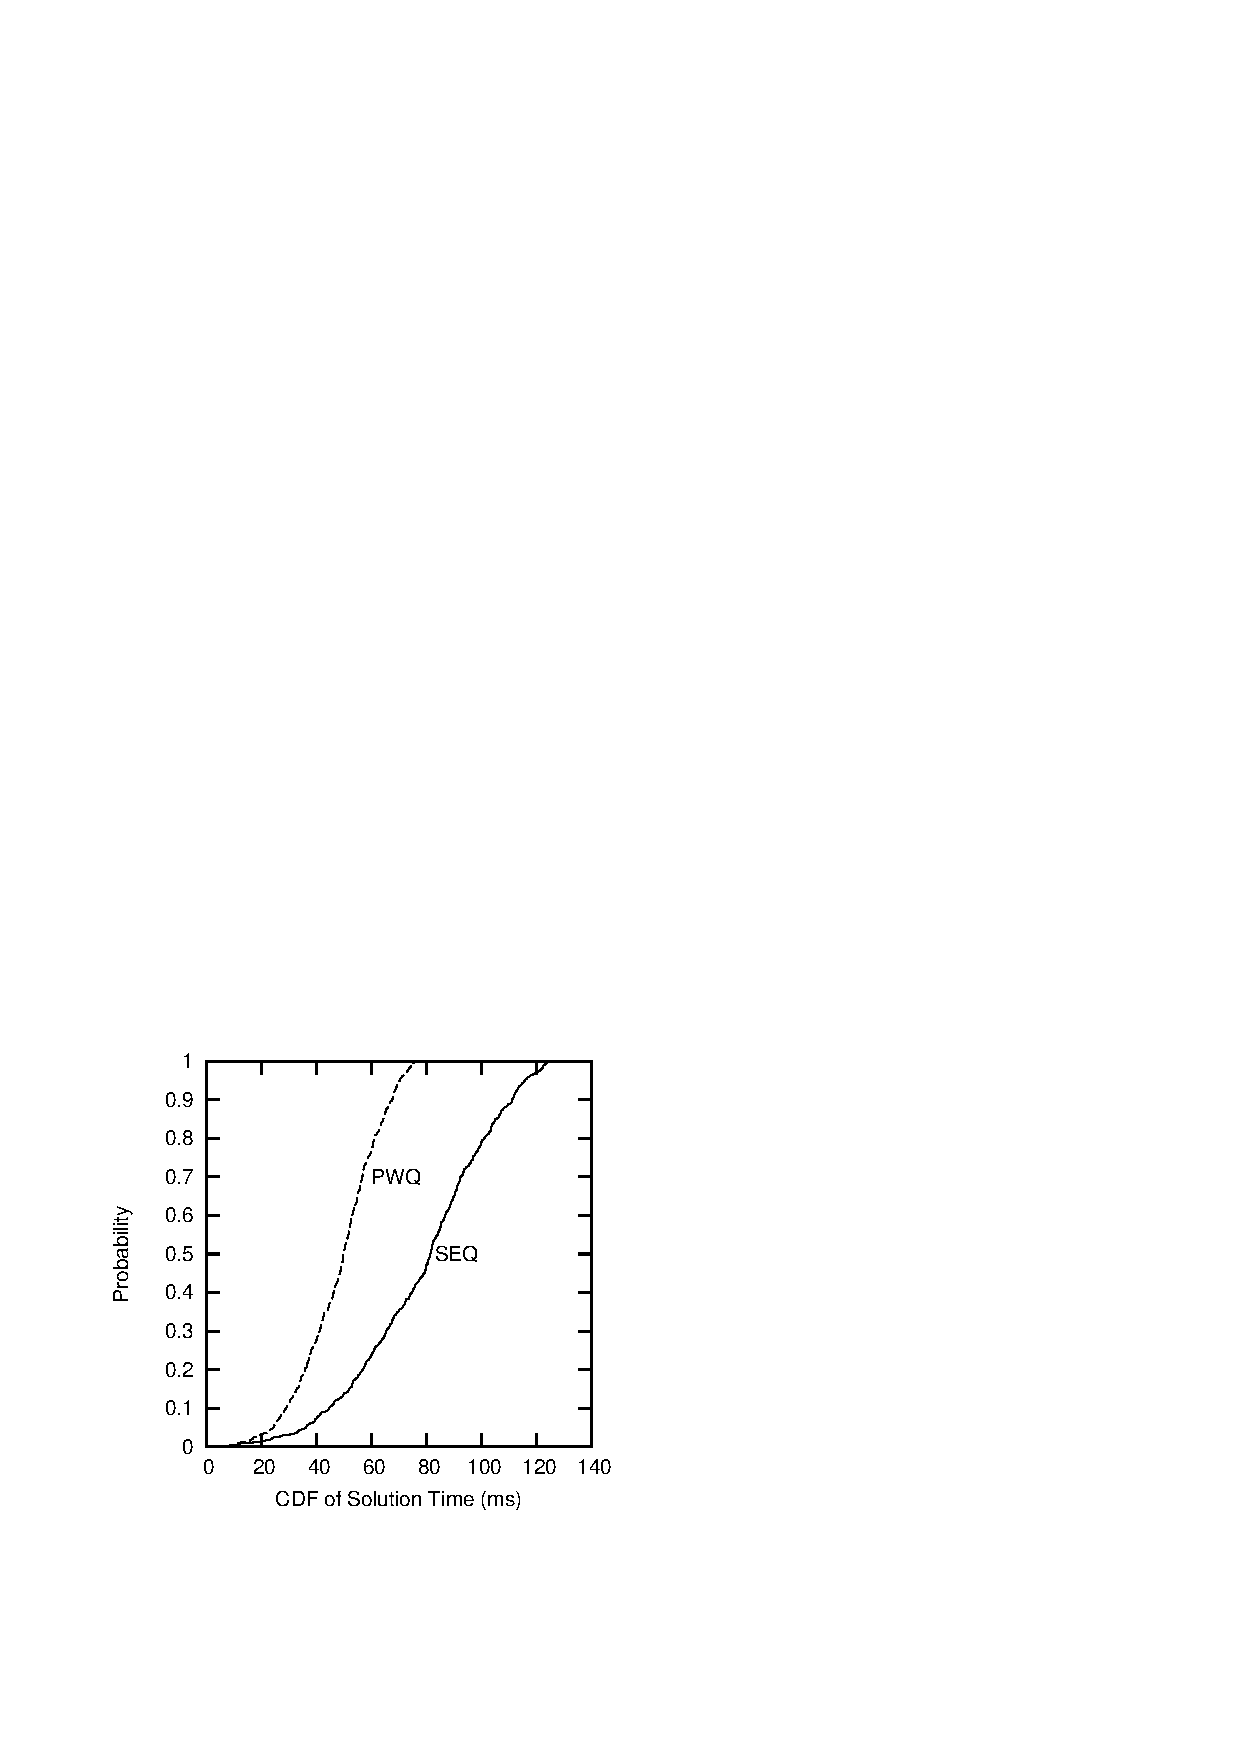
\includegraphics{SMPdesign/500-ms_seq_fg-cdf}}
\caption{CDF of Solution Times For SEQ and PWQ}
\label{fig:SMPdesign:CDF of Solution Times For SEQ and PWQ}
\end{figure}

The parallel work-queue solver is a straightforward parallelization
of the algorithm shown in
Listings~\ref{lst:SMPdesign:SEQ Pseudocode} and~\ref{lst:SMPdesign:SEQ Helper Pseudocode}.
\begin{fcvref}[ln:SMPdesign:SEQ Pseudocode]
\Clnref{ifge} of Listing~\ref{lst:SMPdesign:SEQ Pseudocode} must use fetch-and-add,
and the local variable \co{vi} must be shared among the various threads.
\end{fcvref}
\begin{fcvref}[ln:SMPdesign:SEQ Helper Pseudocode:try]
\Clnref{chk:not:visited,mark:visited} of Listing~\ref{lst:SMPdesign:SEQ Helper Pseudocode} must be
combined into a CAS loop, with CAS failure indicating a loop in the
maze.
\Clnrefrange{recordnext}{next:visited} of this listing must use
fetch-and-add to arbitrate concurrent
attempts to record cells in the \co{->visited[]} array.
\end{fcvref}

This approach does provide significant speedups on a dual-CPU
Lenovo W500 running at 2.53\,GHz, as shown in
Figure~\ref{fig:SMPdesign:CDF of Solution Times For SEQ and PWQ},
which shows the cumulative distribution functions (CDFs) for the solution
times of the two algorithms, based on the solution of 500 different square
500-by-500 randomly generated mazes.
The substantial overlap
of the projection of the CDFs onto the x-axis will be addressed in
Section~\ref{sec:SMPdesign:Performance Comparison I}.

Interestingly enough, the sequential solution-path tracking works unchanged
for the parallel algorithm.
However, this uncovers a significant weakness in the parallel algorithm:
At most one thread may be making progress along the solution path at
any given time.
This weakness is addressed in the next section.

\subsection{Alternative Parallel Maze Solver}
\label{sec:SMPdesign:Alternative Parallel Maze Solver}

Youthful maze solvers are often urged to start at both ends, and
this advice has been repeated more recently in the context of automated
maze solving~\cite{UMD:CMSC433maze}.
This advice amounts to partitioning, which has been a powerful
parallelization strategy
in the context of parallel programming for both operating-system
kernels~\cite{Beck85,Inman85} and
applications~\cite{DavidAPatterson2010TroubleMulticore}.
This section applies this strategy, using two child threads that start
at opposite ends of the solution path, and takes a brief look at the
performance and scalability consequences.

\begin{listing}[tbp]
\begin{fcvlabel}[ln:SMPdesign:Partitioned Parallel Solver Pseudocode]
\begin{VerbatimL}[commandchars=\\\@\$]
int maze_solve_child(maze *mp, cell *visited, cell sc)	\lnlbl@b$
{
	cell c;
	cell n;
	int vi = 0;

	myvisited = visited; myvi = &vi;		\lnlbl@store:ptr$
	c = visited[vi];				\lnlbl@retrieve$
	do {
		while (!maze_find_any_next_cell(mp, c, &n)) {
			if (visited[++vi].row < 0)
				return 0;
			if (READ_ONCE(mp->done))	\lnlbl@chk:done1$
				return 1;
			c = visited[vi];
		}
		do {
			if (READ_ONCE(mp->done))	\lnlbl@chk:done2$
				return 1;
			c = n;
		} while (maze_find_any_next_cell(mp, c, &n));
		c = visited[vi];
	} while (!READ_ONCE(mp->done));		\lnlbl@chk:done3$
	return 1;
}
\end{VerbatimL}
\end{fcvlabel}
\caption{Partitioned Parallel Solver Pseudocode}
\label{lst:SMPdesign:Partitioned Parallel Solver Pseudocode}
\end{listing}

\begin{fcvref}[ln:SMPdesign:Partitioned Parallel Solver Pseudocode]
The partitioned parallel algorithm (PART), shown in
Listing~\ref{lst:SMPdesign:Partitioned Parallel Solver Pseudocode}
(\path{maze_part.c}),
is similar to SEQ, but has a few important differences.
First, each child thread has its own \co{visited} array, passed in by
the parent as shown on line~\lnref{b},
which must be initialized to all [$-1$, $-1$].
Line~\lnref{store:ptr} stores a pointer to this array into the per-thread variable
\co{myvisited} to allow access by helper functions, and similarly stores
a pointer to the local visit index.
Second, the parent visits the first cell on each child's behalf,
which the child retrieves on line~\lnref{retrieve}.
Third, the maze is solved as soon as one child locates a cell that has
been visited by the other child.
When \co{maze_try_visit_cell()} detects this,
it sets a \co{->done} field in the maze structure.
Fourth, each child must therefore periodically check the \co{->done}
field, as shown on lines~\lnref{chk:done1}, \lnref{chk:done2}, and~\lnref{chk:done3}.
The \co{READ_ONCE()} primitive must disable any compiler
optimizations that might combine consecutive loads or that
might reload the value.
A C++1x volatile relaxed load suffices~\cite{RichardSmith2019N4800}.
Finally, the \co{maze_find_any_next_cell()} function must use
compare-and-swap to mark a cell as visited, however
no constraints on ordering are required beyond those provided by
thread creation and join.
\end{fcvref}

\begin{listing}[tbp]
\begin{fcvlabel}[ln:SMPdesign:Partitioned Parallel Helper Pseudocode]
\begin{VerbatimL}[commandchars=\\\@\$]
int maze_try_visit_cell(struct maze *mp, int c, int t,
                        int *n, int d)
{
	cell_t t;
	cell_t *tp;
	int vi;

	if (!maze_cells_connected(mp, c, t))		\lnlbl@chk:conn:b$
		return 0;				\lnlbl@chk:conn:e$
	tp = celladdr(mp, t);
	do {						\lnlbl@loop:b$
		t = READ_ONCE(*tp);
		if (t & VISITED) {			\lnlbl@chk:visited$
			if ((t & TID) != mytid)		\lnlbl@chk:other$
				mp->done = 1;		\lnlbl@located$
			return 0;			\lnlbl@ret:fail$
		}
	} while (!CAS(tp, t, t | VISITED | myid | d));	\lnlbl@loop:e$
	*n = t;						\lnlbl@update:new$
	vi = (*myvi)++;					\lnlbl@update:visited:b$
	myvisited[vi] = t;				\lnlbl@update:visited:e$
	return 1;					\lnlbl@ret:success$
}
\end{VerbatimL}
\end{fcvlabel}
\caption{Partitioned Parallel Helper Pseudocode}
\label{lst:SMPdesign:Partitioned Parallel Helper Pseudocode}
\end{listing}

\begin{fcvref}[ln:SMPdesign:Partitioned Parallel Helper Pseudocode]
The pseudocode for \co{maze_find_any_next_cell()} is identical to that shown in
Listing~\ref{lst:SMPdesign:SEQ Helper Pseudocode},
but the pseudocode for \co{maze_try_visit_cell()} differs, and
is shown in
Listing~\ref{lst:SMPdesign:Partitioned Parallel Helper Pseudocode}.
\Clnrefrange{chk:conn:b}{chk:conn:e}
check to see if the cells are connected, returning failure
if not.
The loop spanning \clnrefrange{loop:b}{loop:e} attempts to mark
the new cell visited.
Line~\lnref{chk:visited} checks to see if it has already been visited, in which case
line~\lnref{ret:fail} returns failure, but only after line~\lnref{chk:other}
checks to see if
we have encountered the other thread, in which case line~\lnref{located} indicates
that the solution has been located.
Line~\lnref{update:new} updates to the new cell,
lines~\lnref{update:visited:b} and~\lnref{update:visited:e} update this thread's visited
array, and line~\lnref{ret:success} returns success.
\end{fcvref}

\begin{figure}[tb]
\centering
\resizebox{2.2in}{!}{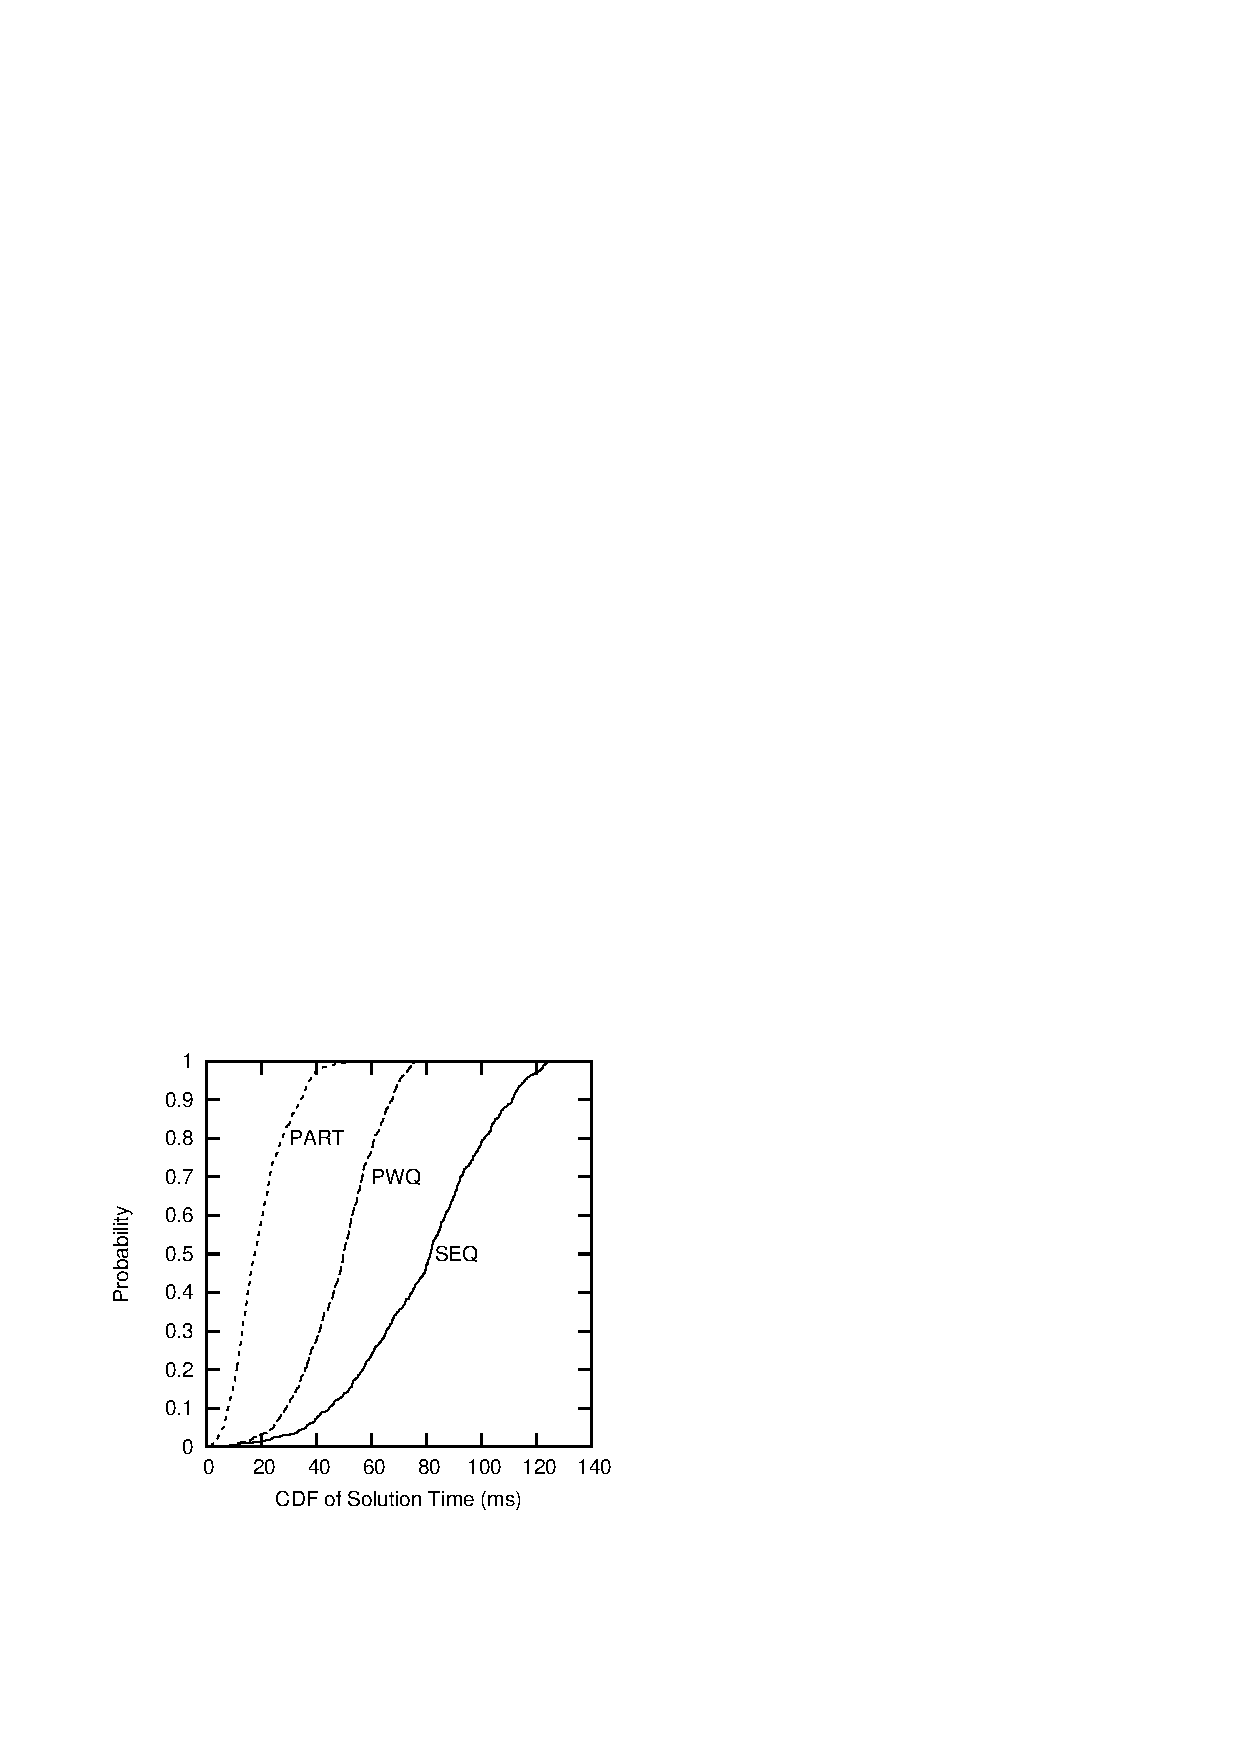
\includegraphics{SMPdesign/500-ms_seq_fg_part-cdf}}
\caption{CDF of Solution Times For SEQ, PWQ, and PART}
\label{fig:SMPdesign:CDF of Solution Times For SEQ, PWQ, and PART}
\end{figure}

Performance testing revealed a surprising anomaly, shown in
Figure~\ref{fig:SMPdesign:CDF of Solution Times For SEQ, PWQ, and PART}.
The median solution time for PART (17 milliseconds)
is more than four times faster than that of SEQ (79 milliseconds),
despite running on only two threads.
The next section analyzes this anomaly.

\subsection{Performance Comparison I}
\label{sec:SMPdesign:Performance Comparison I}

\begin{figure}[tb]
\centering
\resizebox{2.2in}{!}{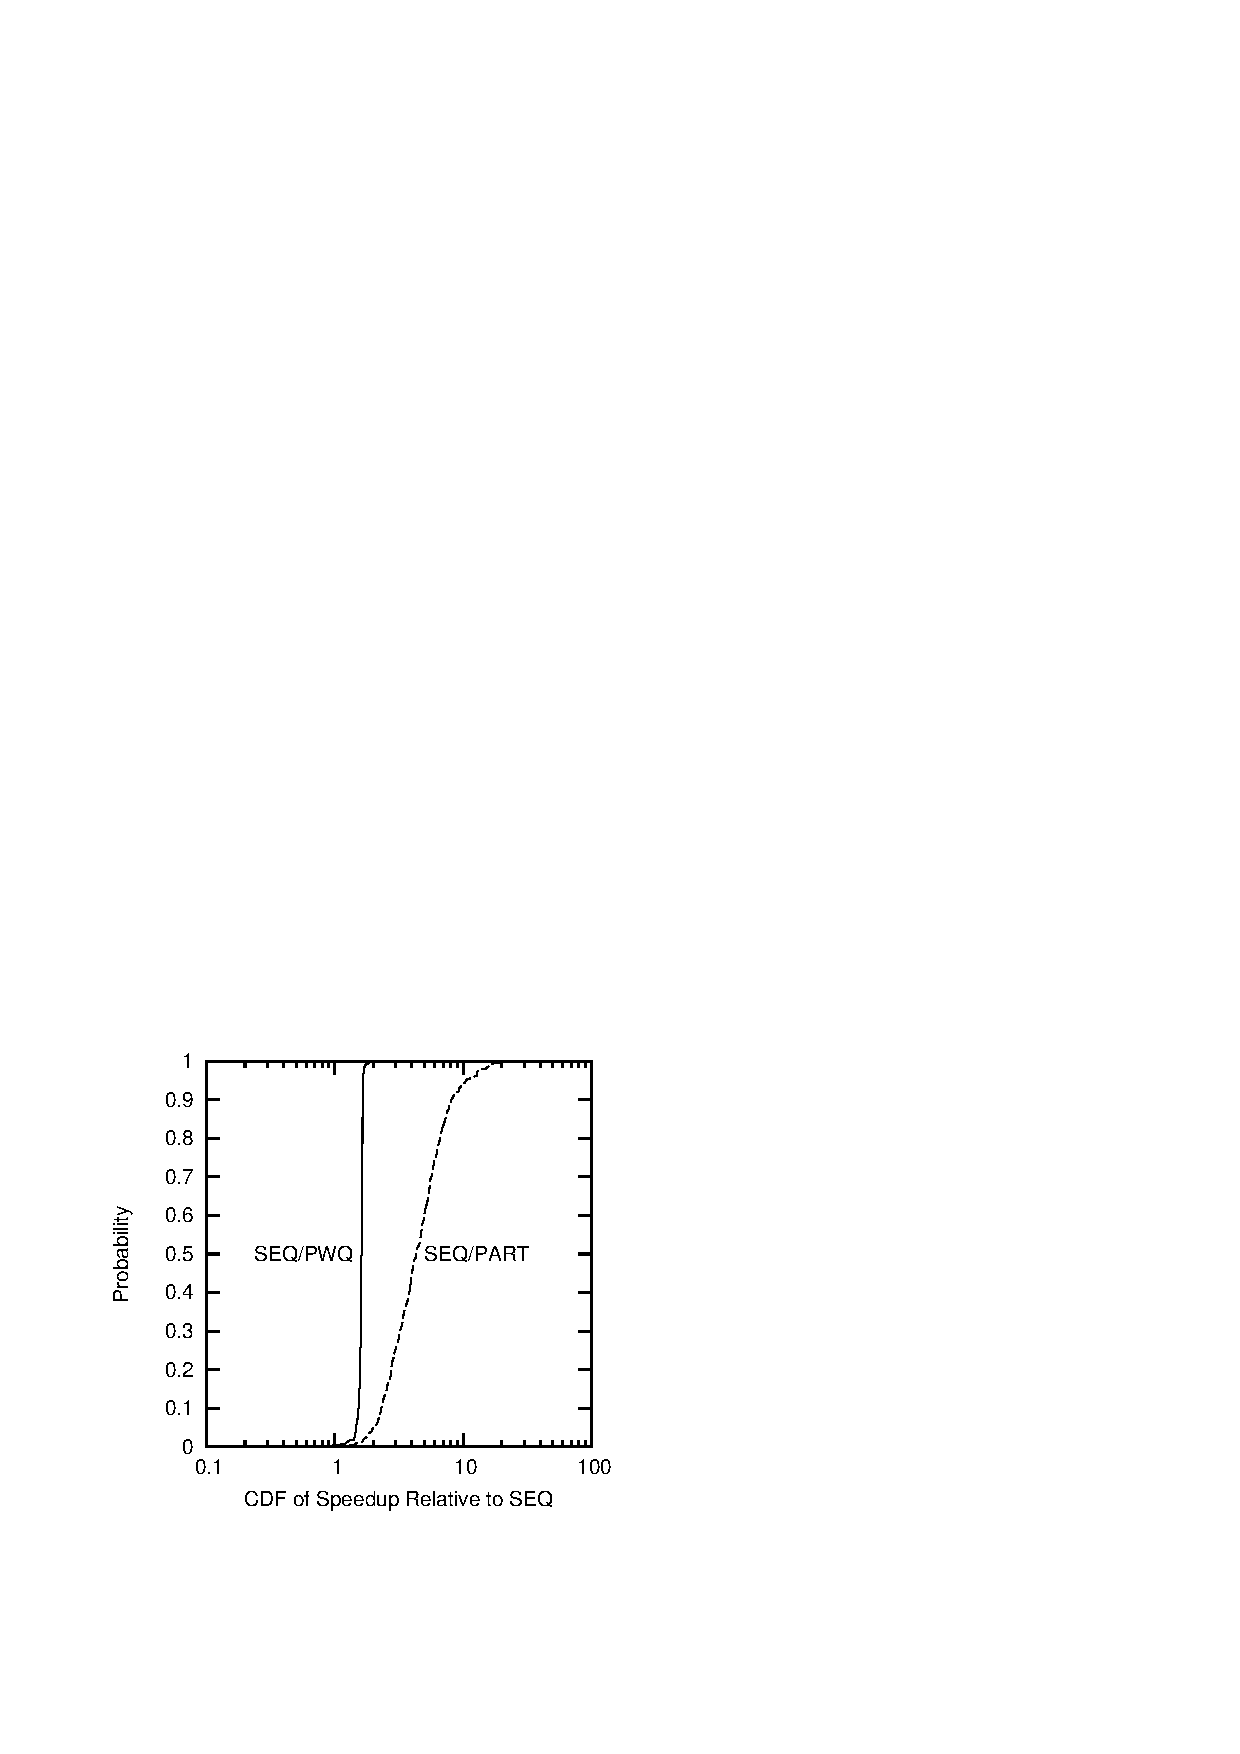
\includegraphics{SMPdesign/500-ms_seqVfg_part-cdf}}
\caption{CDF of SEQ/PWQ and SEQ/PART Solution-Time Ratios}
\label{fig:SMPdesign:CDF of SEQ/PWQ and SEQ/PART Solution-Time Ratios}
\end{figure}

The first reaction to a performance anomaly is to check for bugs.
Although the algorithms were in fact finding valid solutions, the
plot of CDFs in
Figure~\ref{fig:SMPdesign:CDF of Solution Times For SEQ, PWQ, and PART}
assumes independent data points.
This is not the case:  The performance tests randomly generate a maze,
and then run all solvers on that maze.
It therefore makes sense to plot the CDF of the ratios of
solution times for each generated maze,
as shown in
Figure~\ref{fig:SMPdesign:CDF of SEQ/PWQ and SEQ/PART Solution-Time Ratios},
greatly reducing the CDFs' overlap.
This plot reveals that for some mazes, PART
is more than \emph{forty} times faster than SEQ\@.
In contrast, PWQ is never more than about
two times faster than SEQ\@.
A forty-times speedup on two threads demands explanation.
After all, this is not merely embarrassingly parallel, where partitionability
means that adding threads does not increase the overall computational cost.
It is instead \emph{humiliatingly parallel}: Adding threads
significantly reduces the overall computational cost, resulting in
large algorithmic superlinear speedups.

\begin{figure}[tb]
\centering
\resizebox{1.4in}{!}{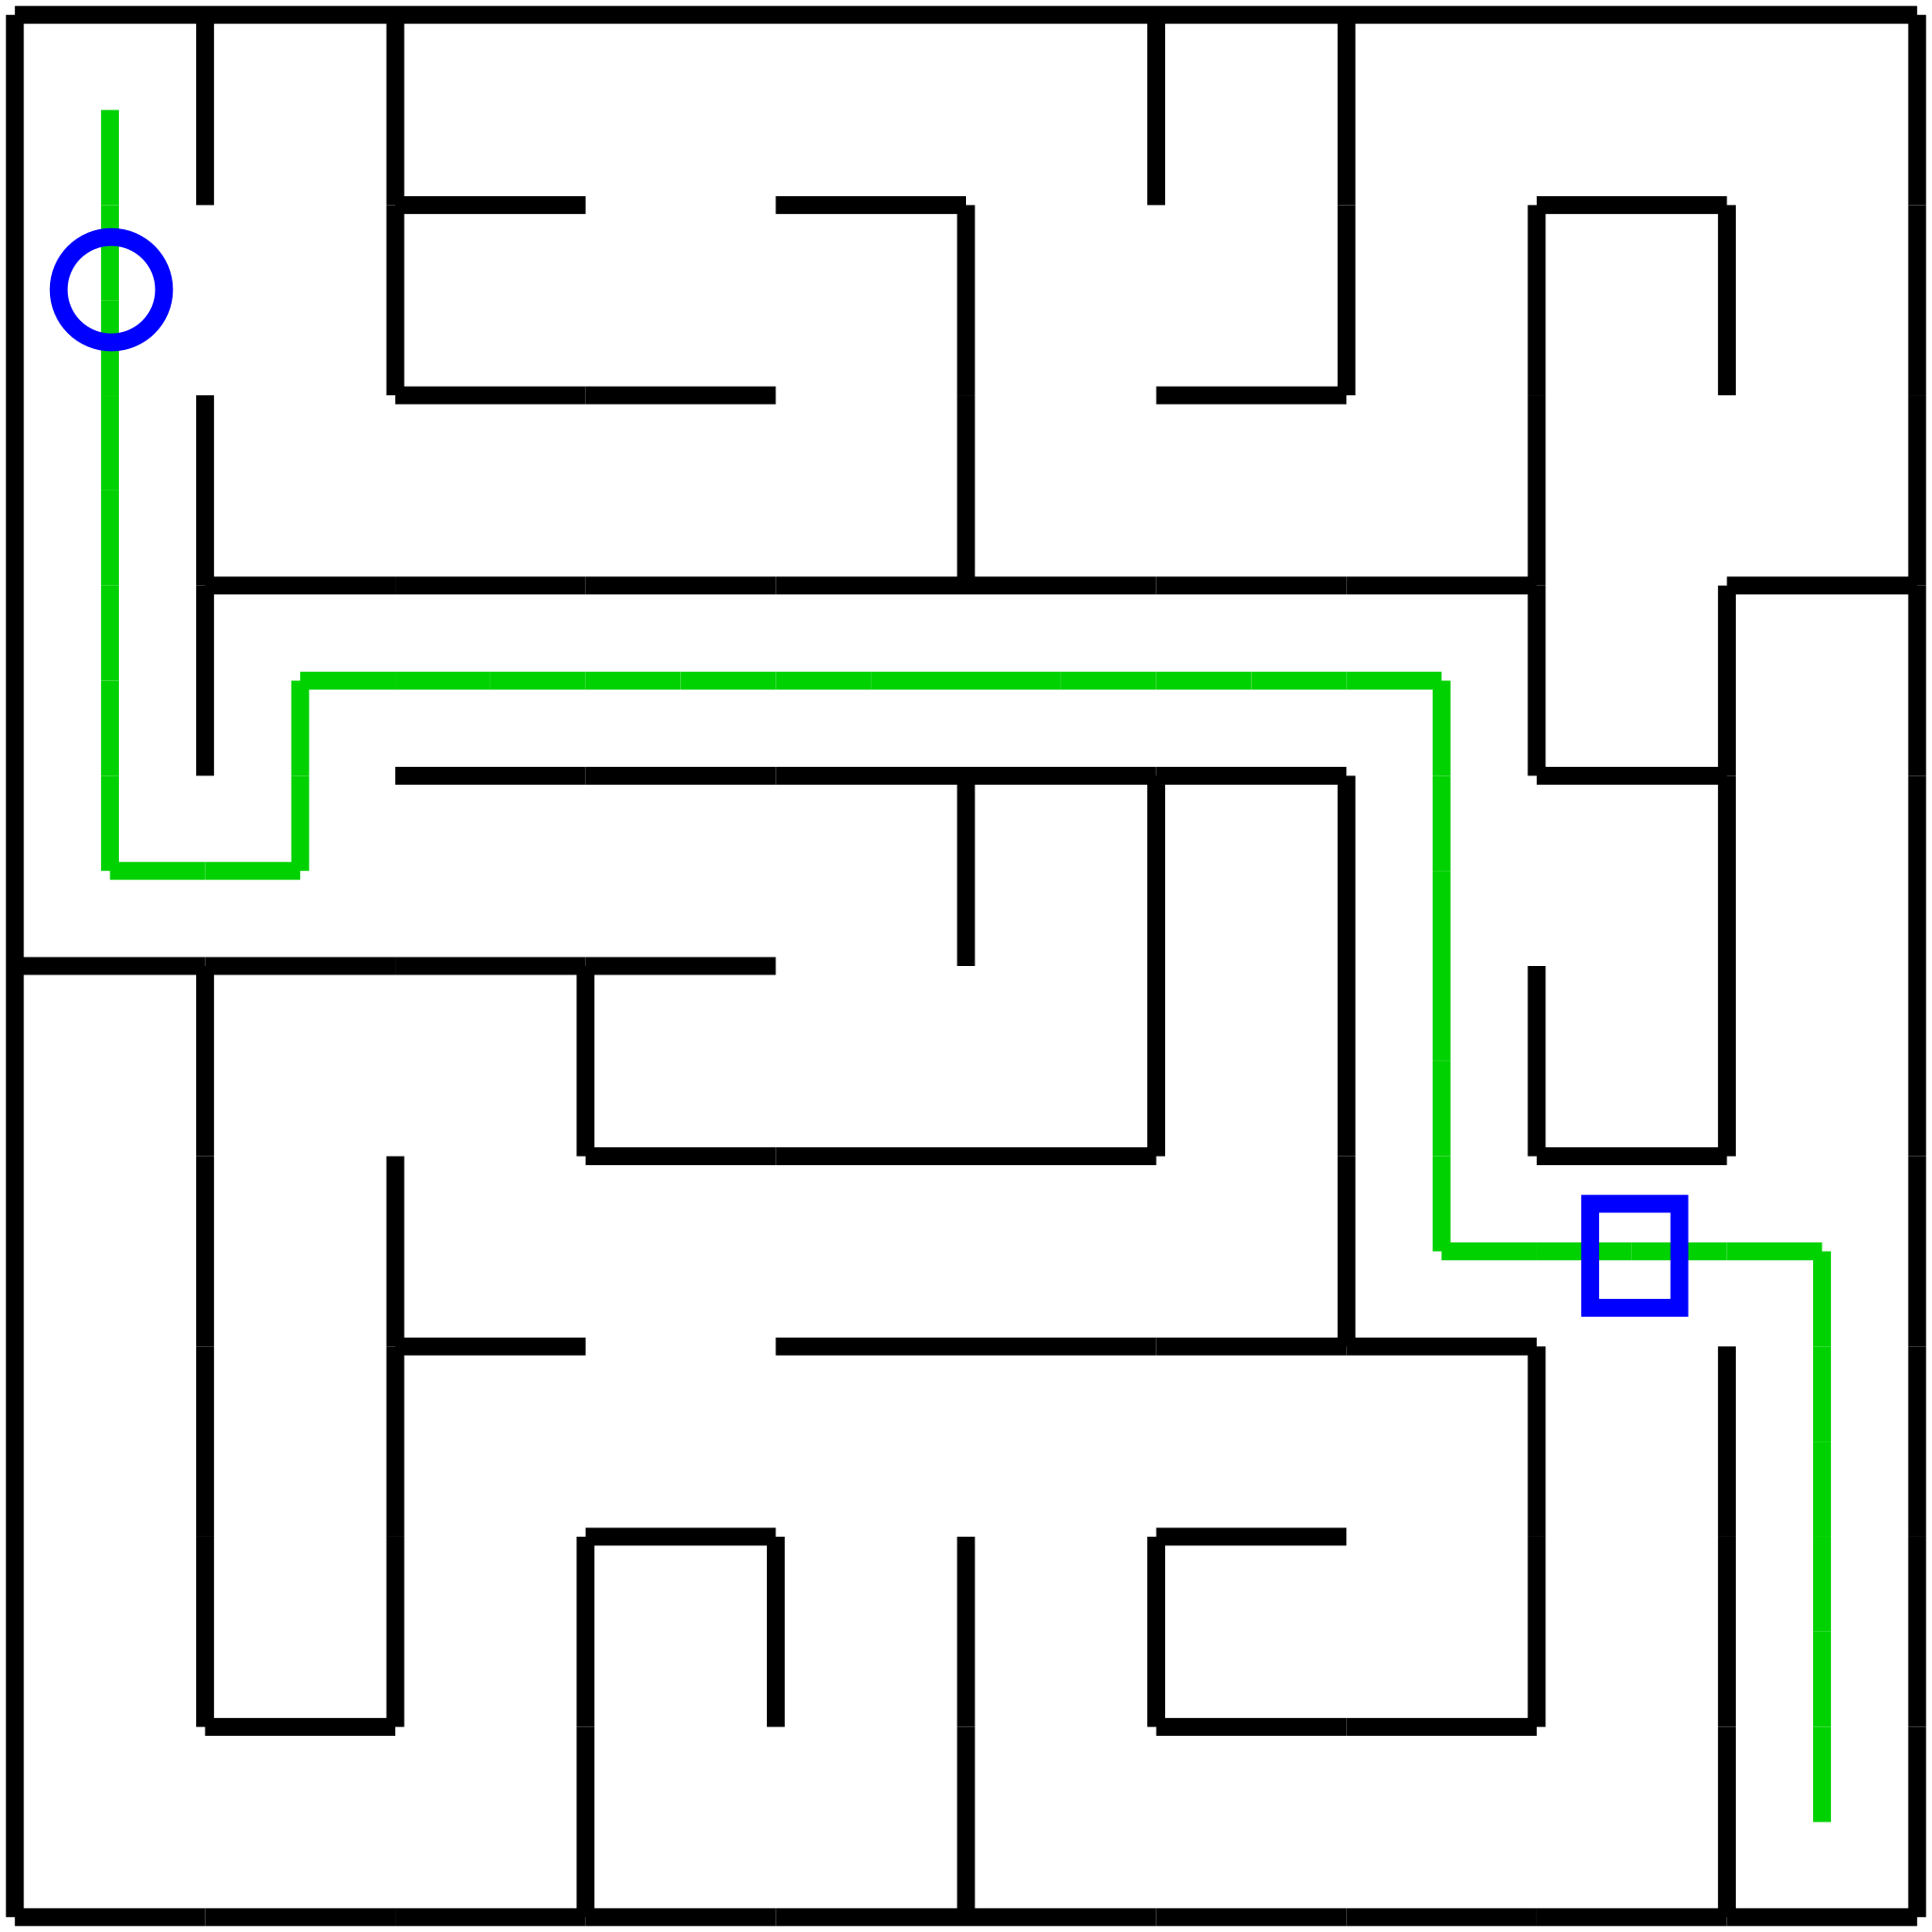
\includegraphics{SMPdesign/maze_in_way10a}}
\caption{Reason for Small Visit Percentages}
\label{fig:SMPdesign:Reason for Small Visit Percentages}
\end{figure}

\begin{figure}[tb]
\centering
\resizebox{2.2in}{!}{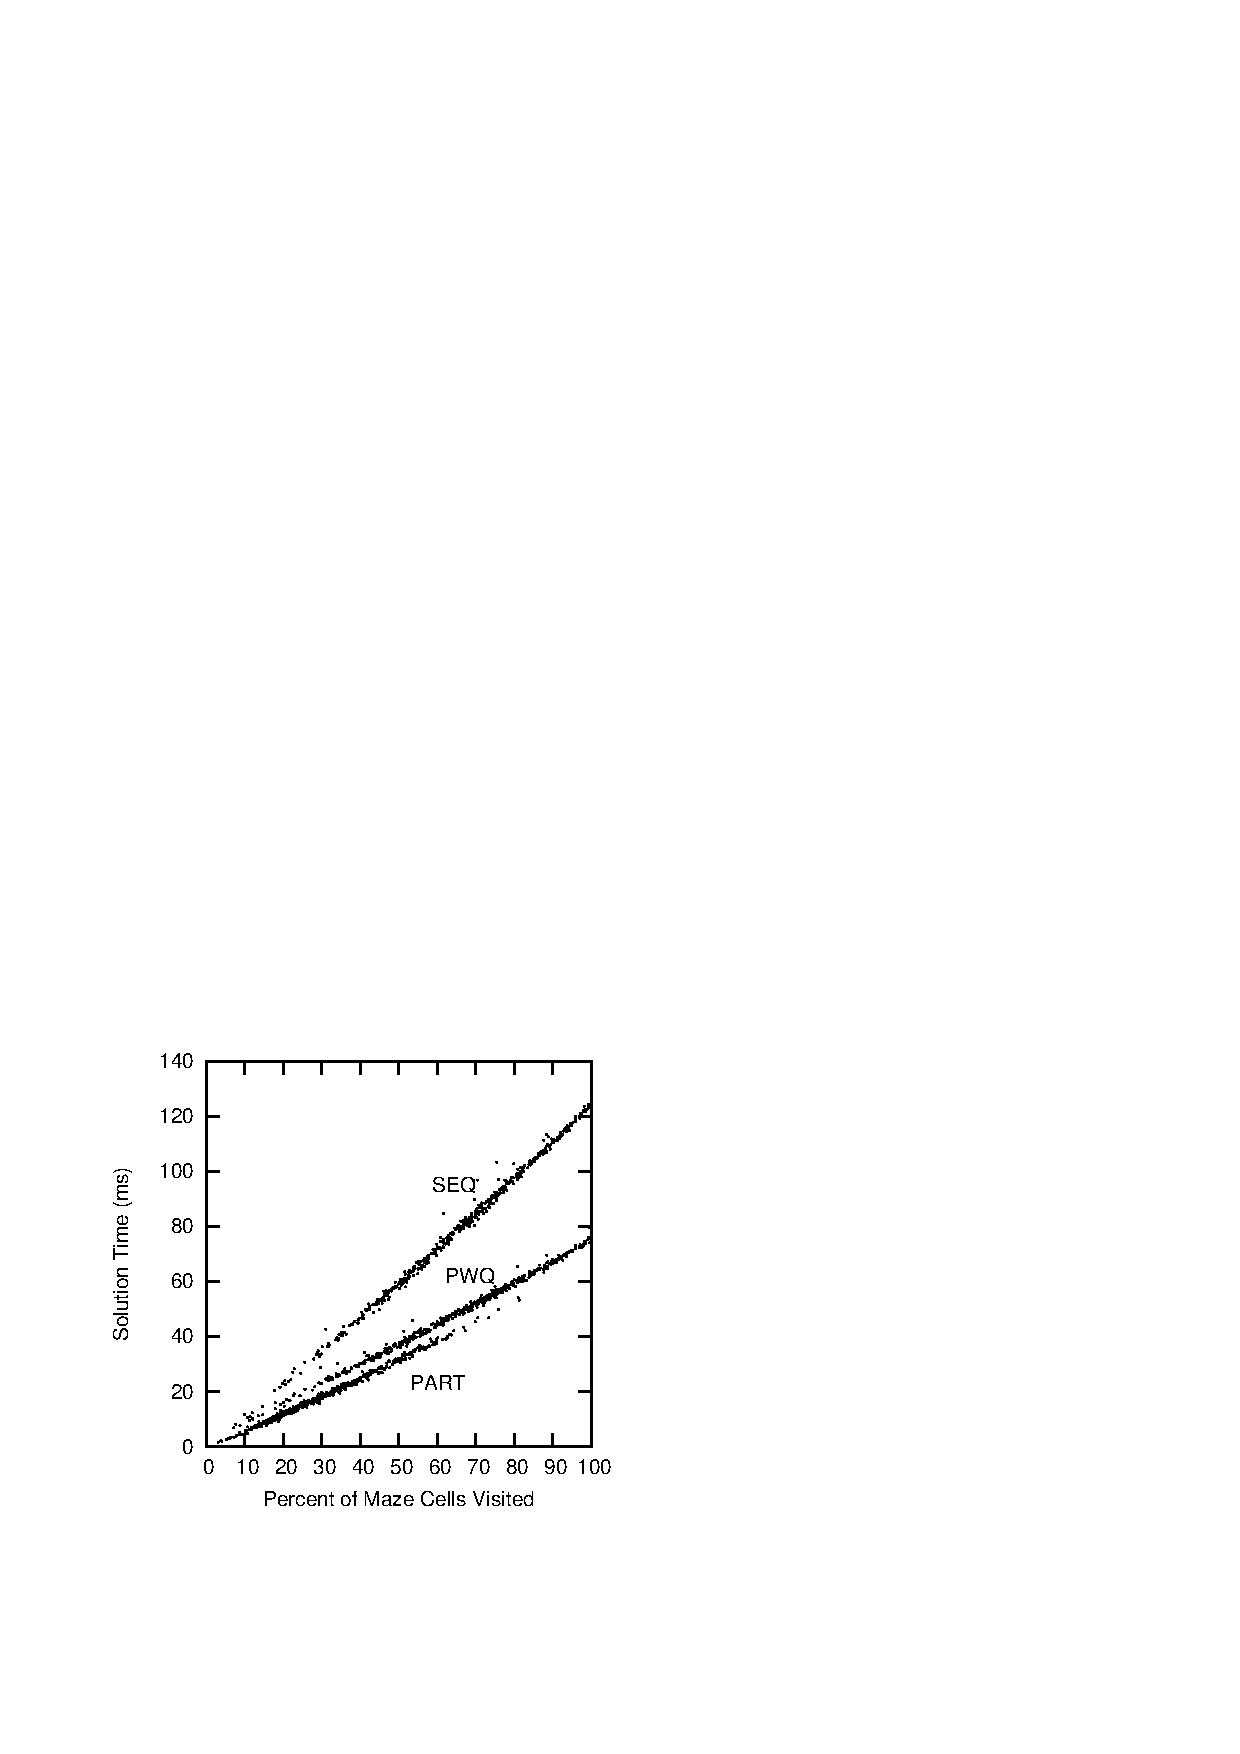
\includegraphics{SMPdesign/500-pctVms_seq_part-sct}}
\caption{Correlation Between Visit Percentage and Solution Time}
\label{fig:SMPdesign:Correlation Between Visit Percentage and Solution Time}
\end{figure}

Further investigation showed that
PART sometimes visited fewer than 2\,\% of the maze's cells,
while SEQ and PWQ never visited fewer than about 9\,\%.
The reason for this difference is shown by
Figure~\ref{fig:SMPdesign:Reason for Small Visit Percentages}.
If the thread traversing the solution from the upper left reaches
the circle, the other thread cannot reach
the upper-right portion of the maze.
Similarly, if the other thread reaches the square,
the first thread cannot reach the lower-left
portion of the maze.
Therefore, PART will likely visit a small fraction
of the non-solution-path cells.
In short, the superlinear speedups are due to threads getting in each
others' way.
This is a sharp contrast with decades of experience with
parallel programming, where workers have struggled
to keep threads \emph{out} of each others' way.

Figure~\ref{fig:SMPdesign:Correlation Between Visit Percentage and Solution Time}
confirms a strong correlation between cells visited and solution time
for all three methods.
The slope of PART's scatterplot is smaller than that of SEQ,
indicating that PART's pair of threads visits a given fraction
of the maze faster than can SEQ's single thread.
PART's scatterplot is also weighted toward small visit
percentages, confirming that PART does less total work, hence
the observed humiliating parallelism.

\begin{figure}[tb]
\centering
\resizebox{1.4in}{!}{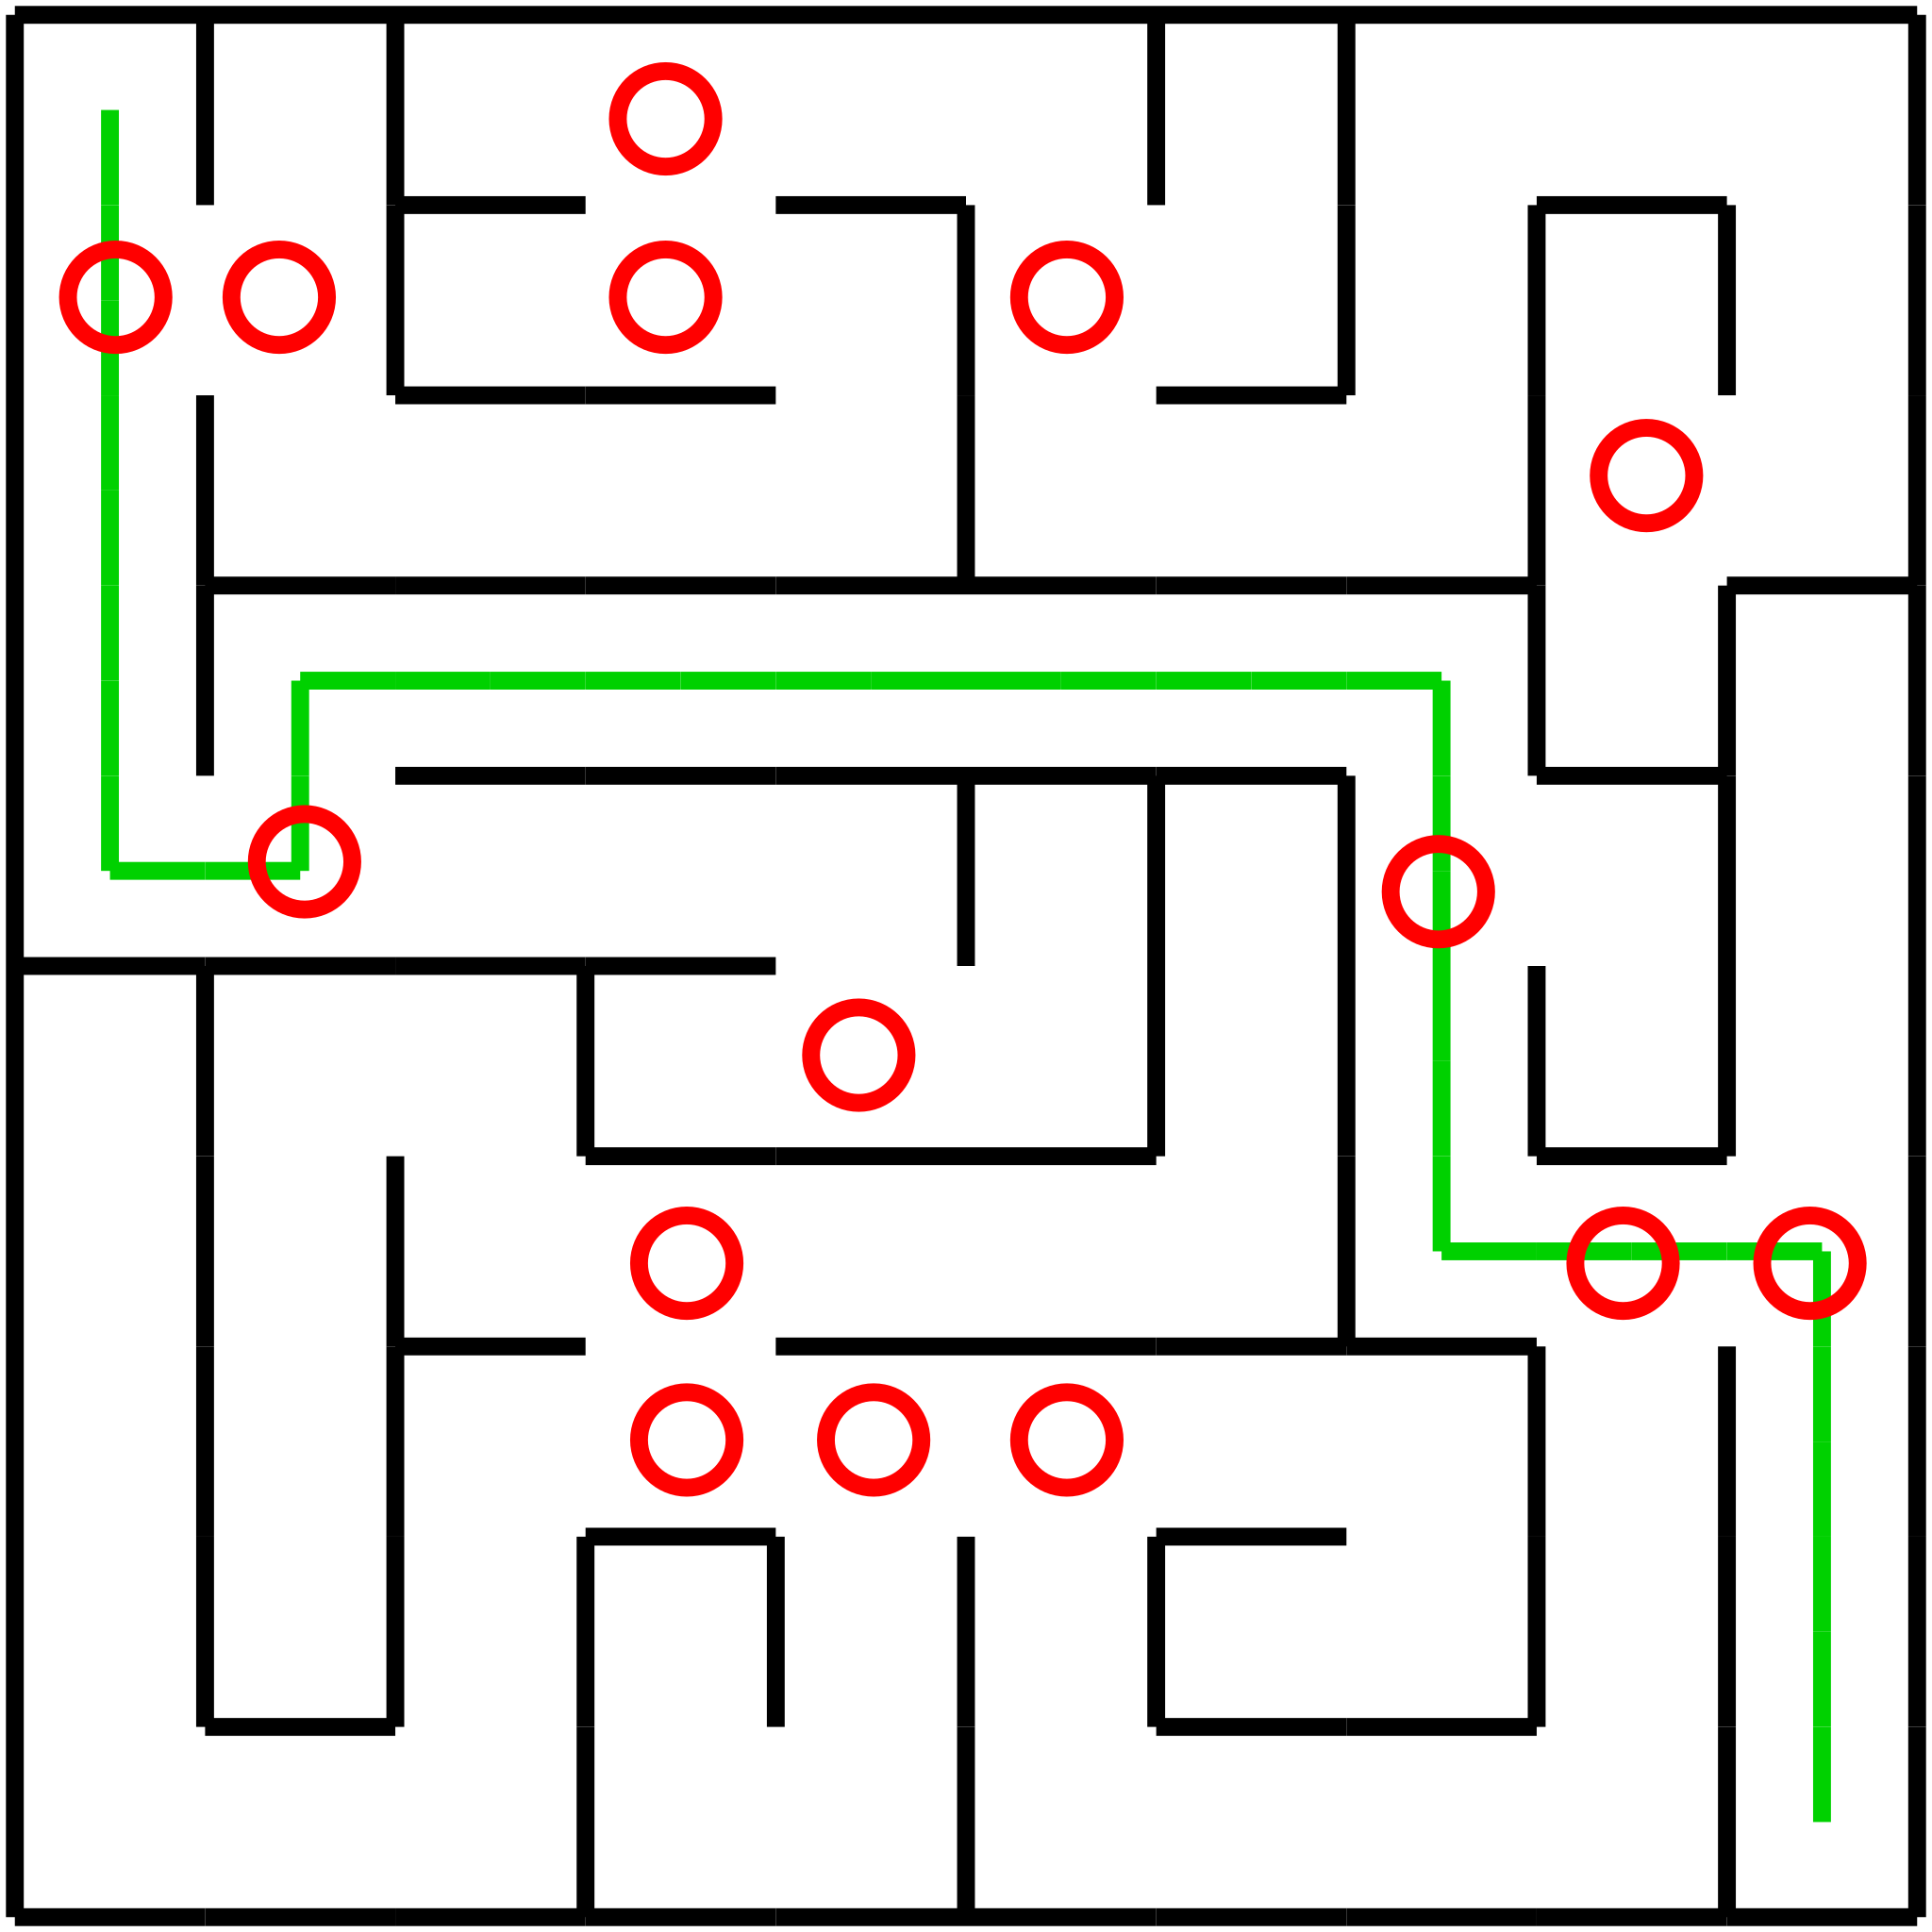
\includegraphics{SMPdesign/maze_PWQ_vs_PART}}
\caption{PWQ Potential Contention Points}
\label{fig:SMPdesign:PWQ Potential Contention Points}
\end{figure}

The fraction of cells visited by PWQ is similar to that of SEQ\@.
In addition, PWQ's solution time is greater than that of PART,
even for equal visit fractions.
The reason for this is shown in
Figure~\ref{fig:SMPdesign:PWQ Potential Contention Points}, which has a red
circle on each cell with more than two neighbors.
Each such cell can result in contention in PWQ, because
one thread can enter but two threads can exit, which hurts
performance, as noted earlier in this chapter.
In contrast, PART can incur such contention but once, namely
when the solution is located.
Of course, SEQ never contends.

\begin{figure}[tb]
\centering
\resizebox{2.2in}{!}{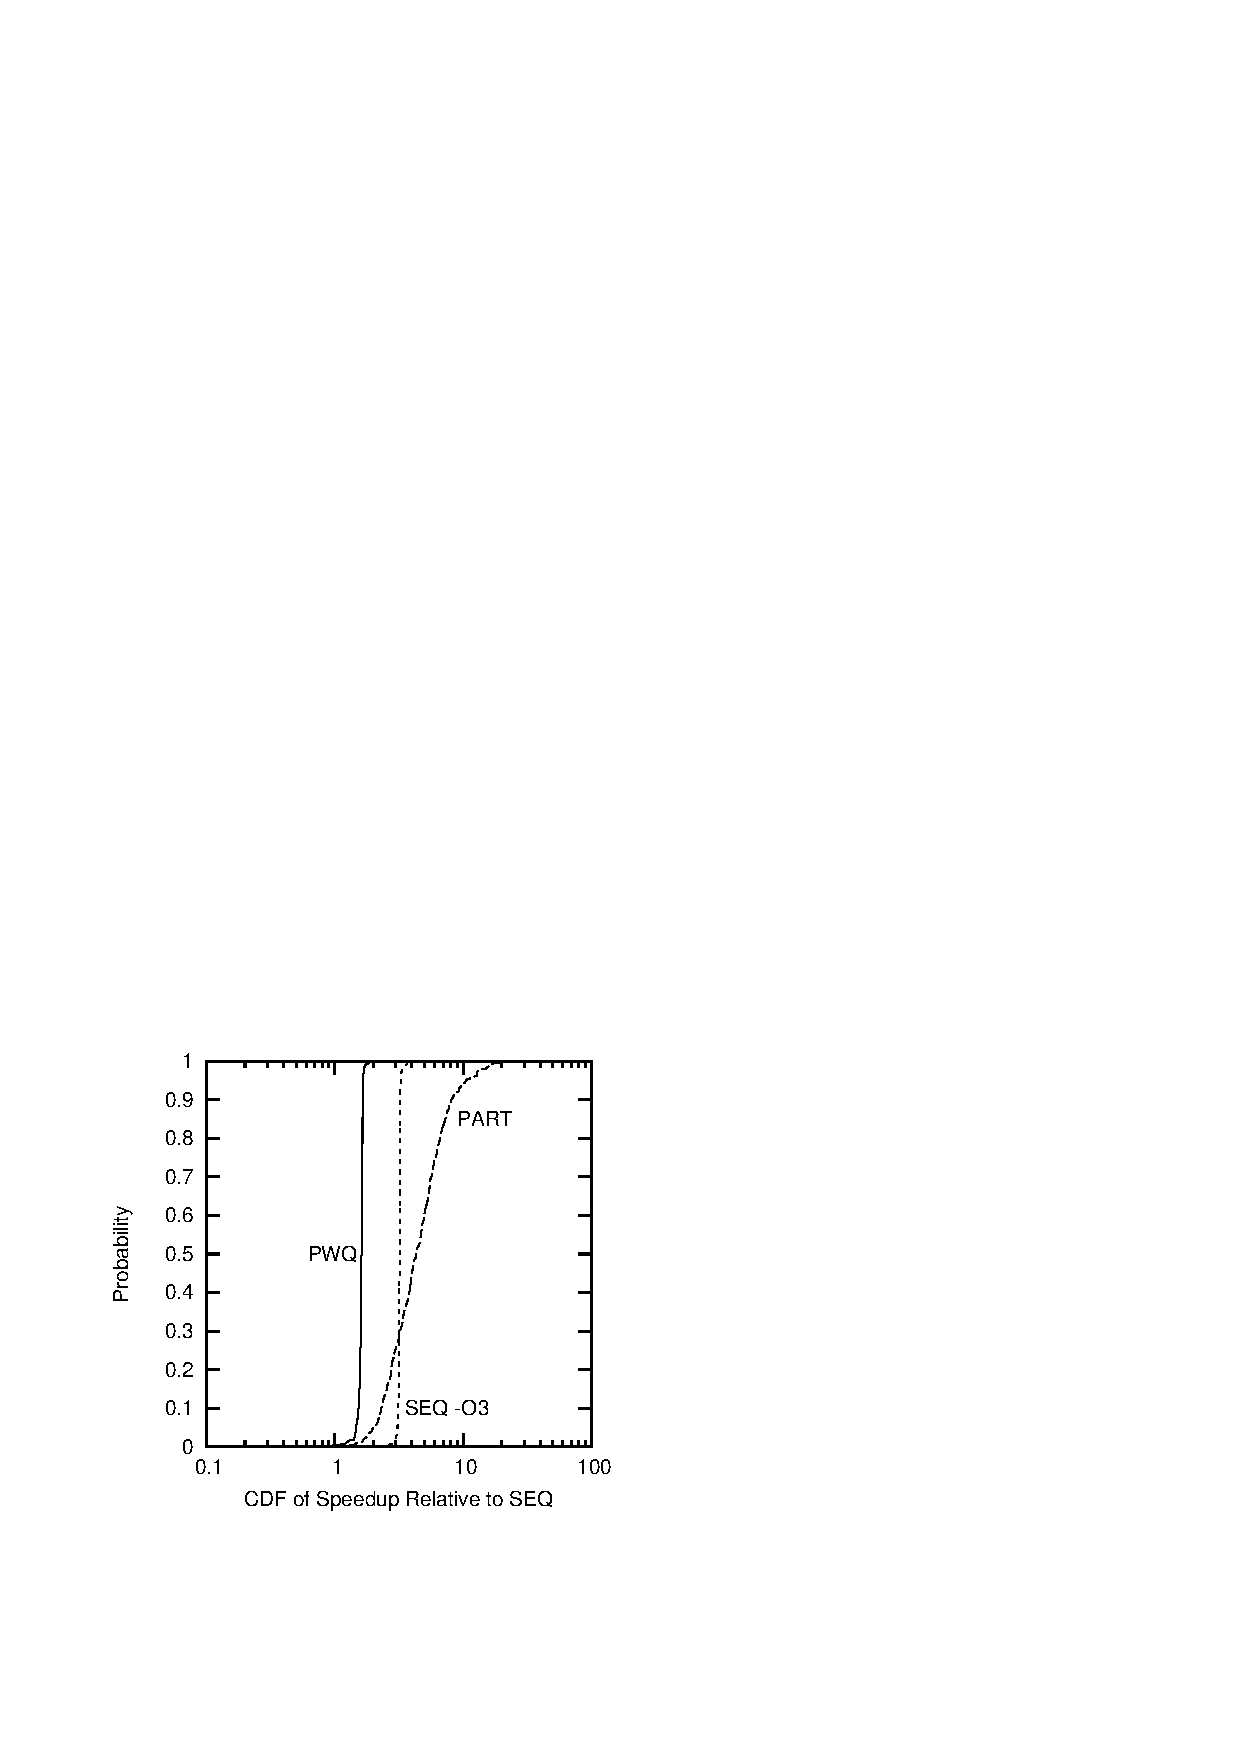
\includegraphics{SMPdesign/500-ms_seqVfg_part_seqO3-cdf}}
\caption{Effect of Compiler Optimization (-O3)}
\label{fig:SMPdesign:Effect of Compiler Optimization (-O3)}
\end{figure}

Although PART's speedup is impressive, we should not neglect sequential
optimizations.
Figure~\ref{fig:SMPdesign:Effect of Compiler Optimization (-O3)} shows that
SEQ, when compiled with -O3, is about twice as fast
as unoptimized PWQ, approaching the performance of unoptimized PART\@.
Compiling all three algorithms with -O3 gives results similar to
(albeit faster than) those shown in
Figure~\ref{fig:SMPdesign:CDF of SEQ/PWQ and SEQ/PART Solution-Time Ratios},
except that PWQ provides almost no speedup compared
to SEQ, in keeping with Amdahl's Law~\cite{GeneAmdahl1967AmdahlsLaw}.
However, if the goal is to double performance compared to unoptimized
SEQ, as opposed to achieving optimality, compiler
optimizations are quite attractive.

Cache alignment and padding often improves performance by reducing
false sharing.
However, for these maze-solution algorithms, aligning and padding the
maze-cell array \emph{degrades} performance by up to 42\,\% for 1000x1000 mazes.
Cache locality is more important than avoiding
false sharing, especially for large mazes.
For smaller 20-by-20 or 50-by-50 mazes, aligning and padding can produce
up to a 40\,\% performance improvement for PART,
but for these small sizes, SEQ performs better anyway because there
is insufficient time for PART to make up for the overhead of
thread creation and destruction.

In short, the partitioned parallel maze solver is an interesting example
of an algorithmic superlinear speedup.
If ``algorithmic superlinear speedup'' causes cognitive dissonance,
please proceed to the next section.

\subsection{Alternative Sequential Maze Solver}
\label{sec:SMPdesign:Alternative Sequential Maze Solver}

\begin{figure}[tb]
\centering
\resizebox{2.2in}{!}{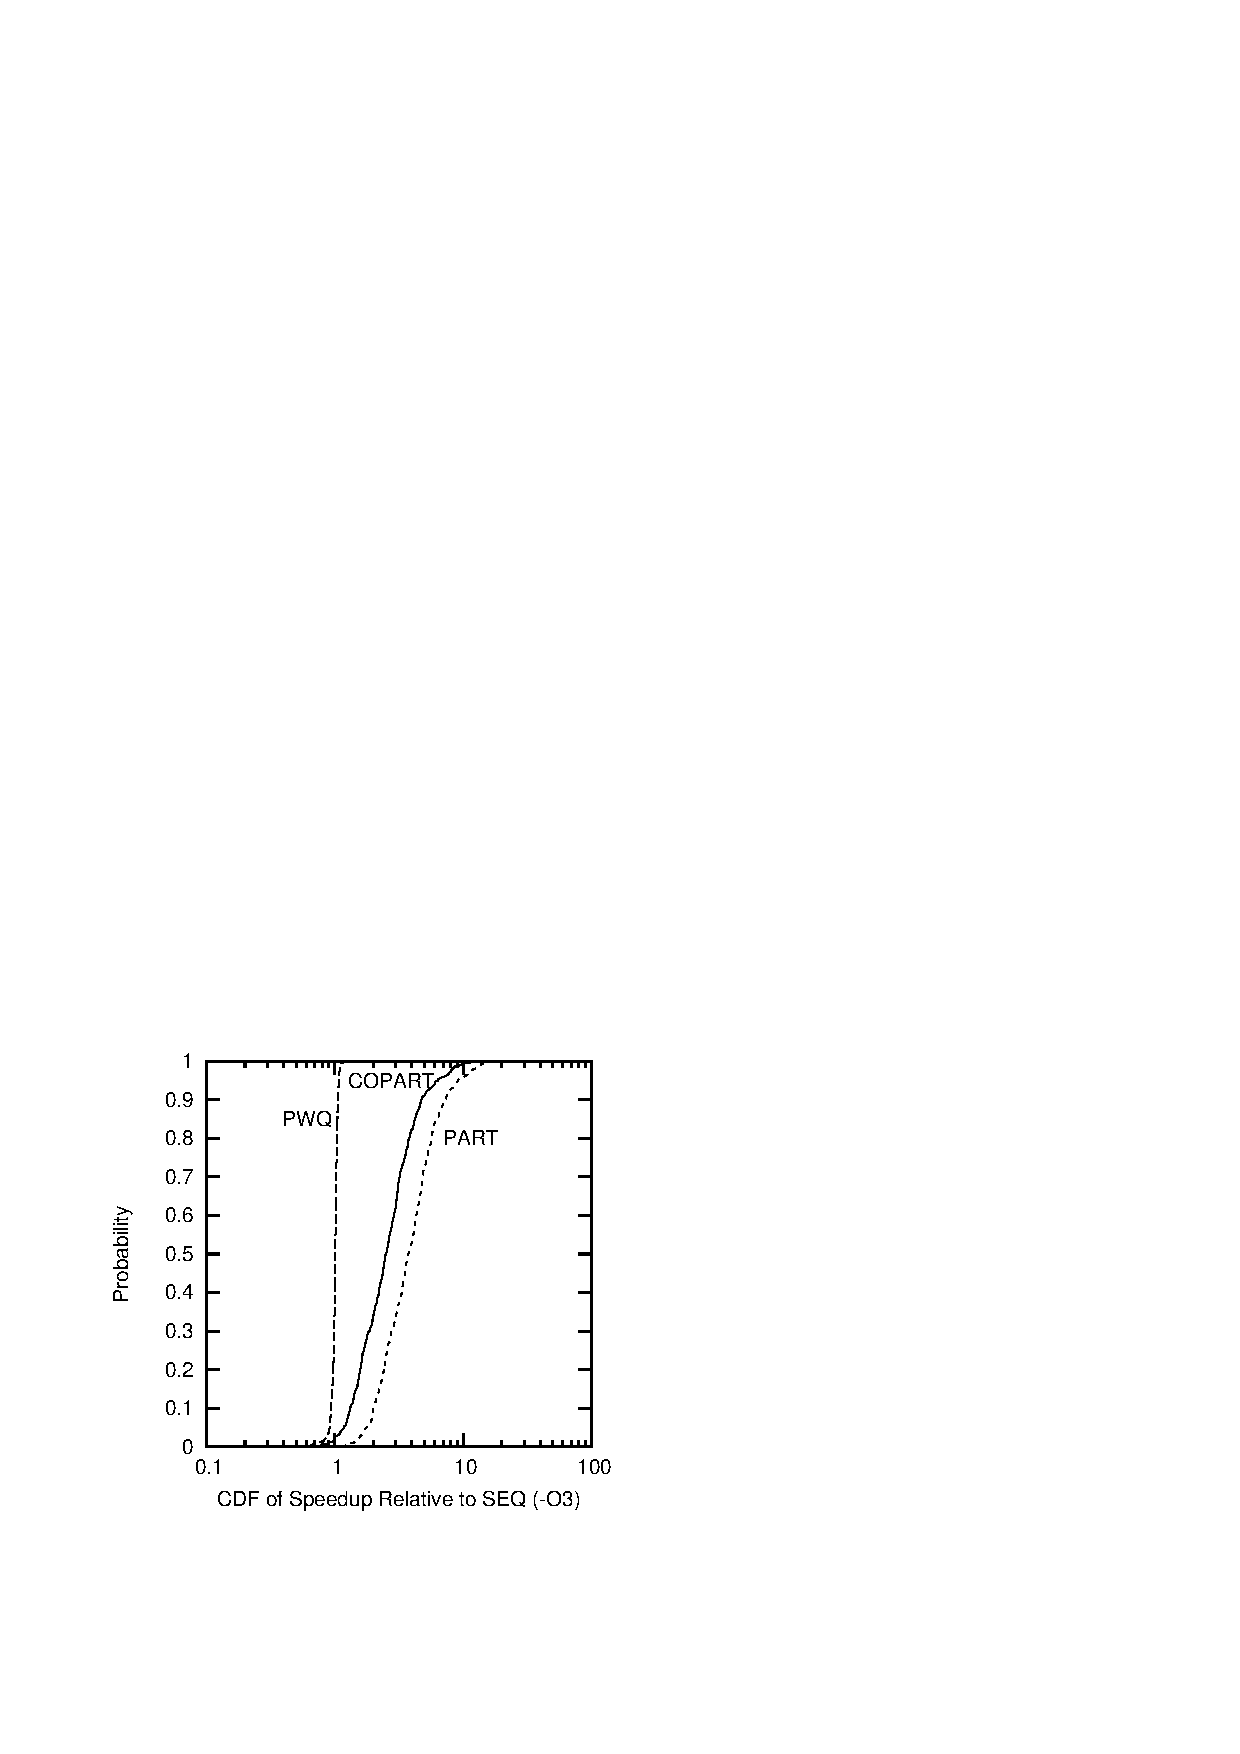
\includegraphics{SMPdesign/500-ms_seqO3V2seqO3_fgO3_partO3-cdf}}
\caption{Partitioned Coroutines}
\label{fig:SMPdesign:Partitioned Coroutines}
\end{figure}

The presence of algorithmic superlinear speedups suggests simulating
parallelism via co-routines, for example, manually switching context
between threads on each pass through the main do-while loop in
Listing~\ref{lst:SMPdesign:Partitioned Parallel Solver Pseudocode}.
This context switching is straightforward because the context
consists only of the variables \co{c} and \co{vi}: Of the numerous
ways to achieve the effect, this is a good tradeoff between
context-switch overhead and visit percentage.
As can be seen in
Figure~\ref{fig:SMPdesign:Partitioned Coroutines},
this coroutine algorithm (COPART) is quite effective, with the performance
on one thread being within about 30\,\% of PART on two threads
(\path{maze_2seq.c}).

\subsection{Performance Comparison II}
\label{sec:SMPdesign:Performance Comparison II}

\begin{figure}[tb]
\centering
\resizebox{2.2in}{!}{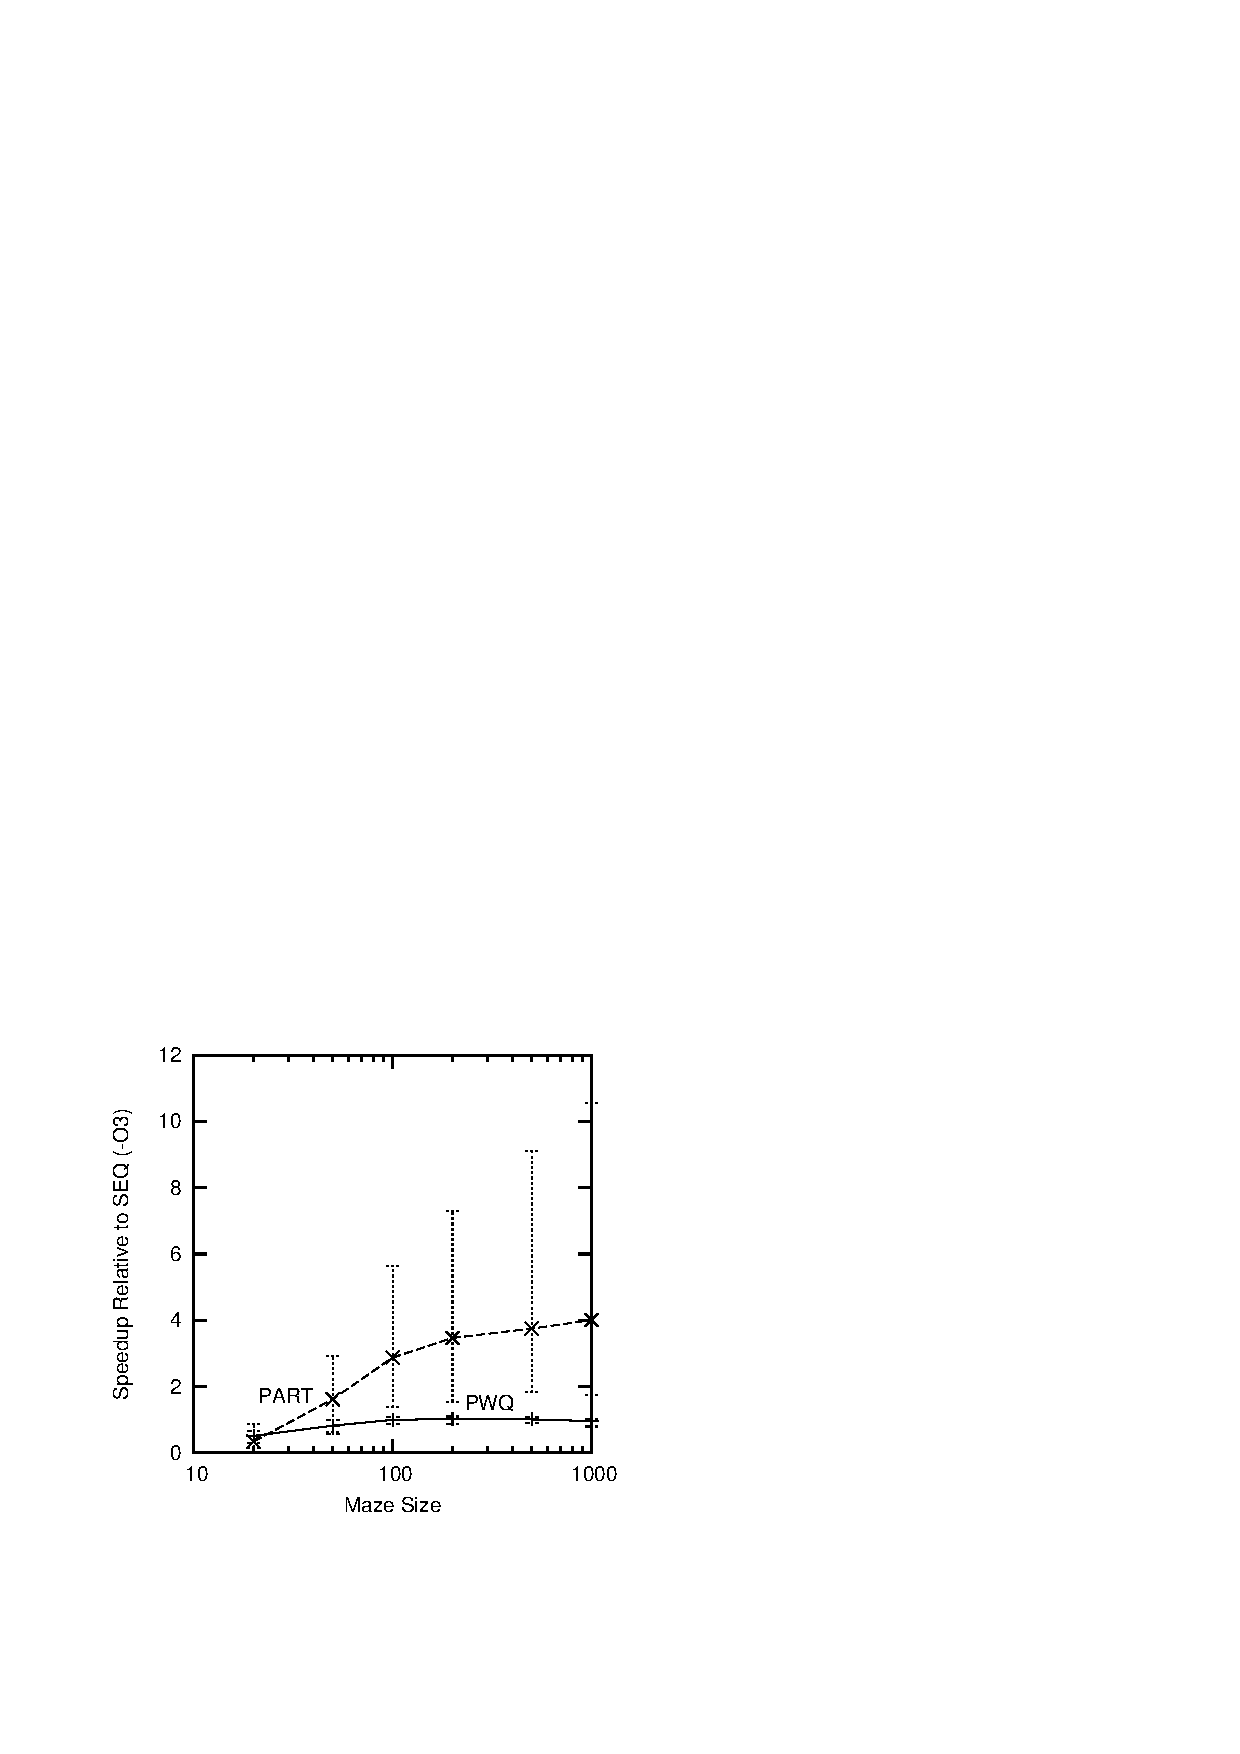
\includegraphics{SMPdesign/500-ms_seqO3VfgO3_partO3-median}}
\caption{Varying Maze Size vs. SEQ}
\label{fig:SMPdesign:Varying Maze Size vs. SEQ}
\end{figure}

\begin{figure}[tb]
\centering
\resizebox{2.2in}{!}{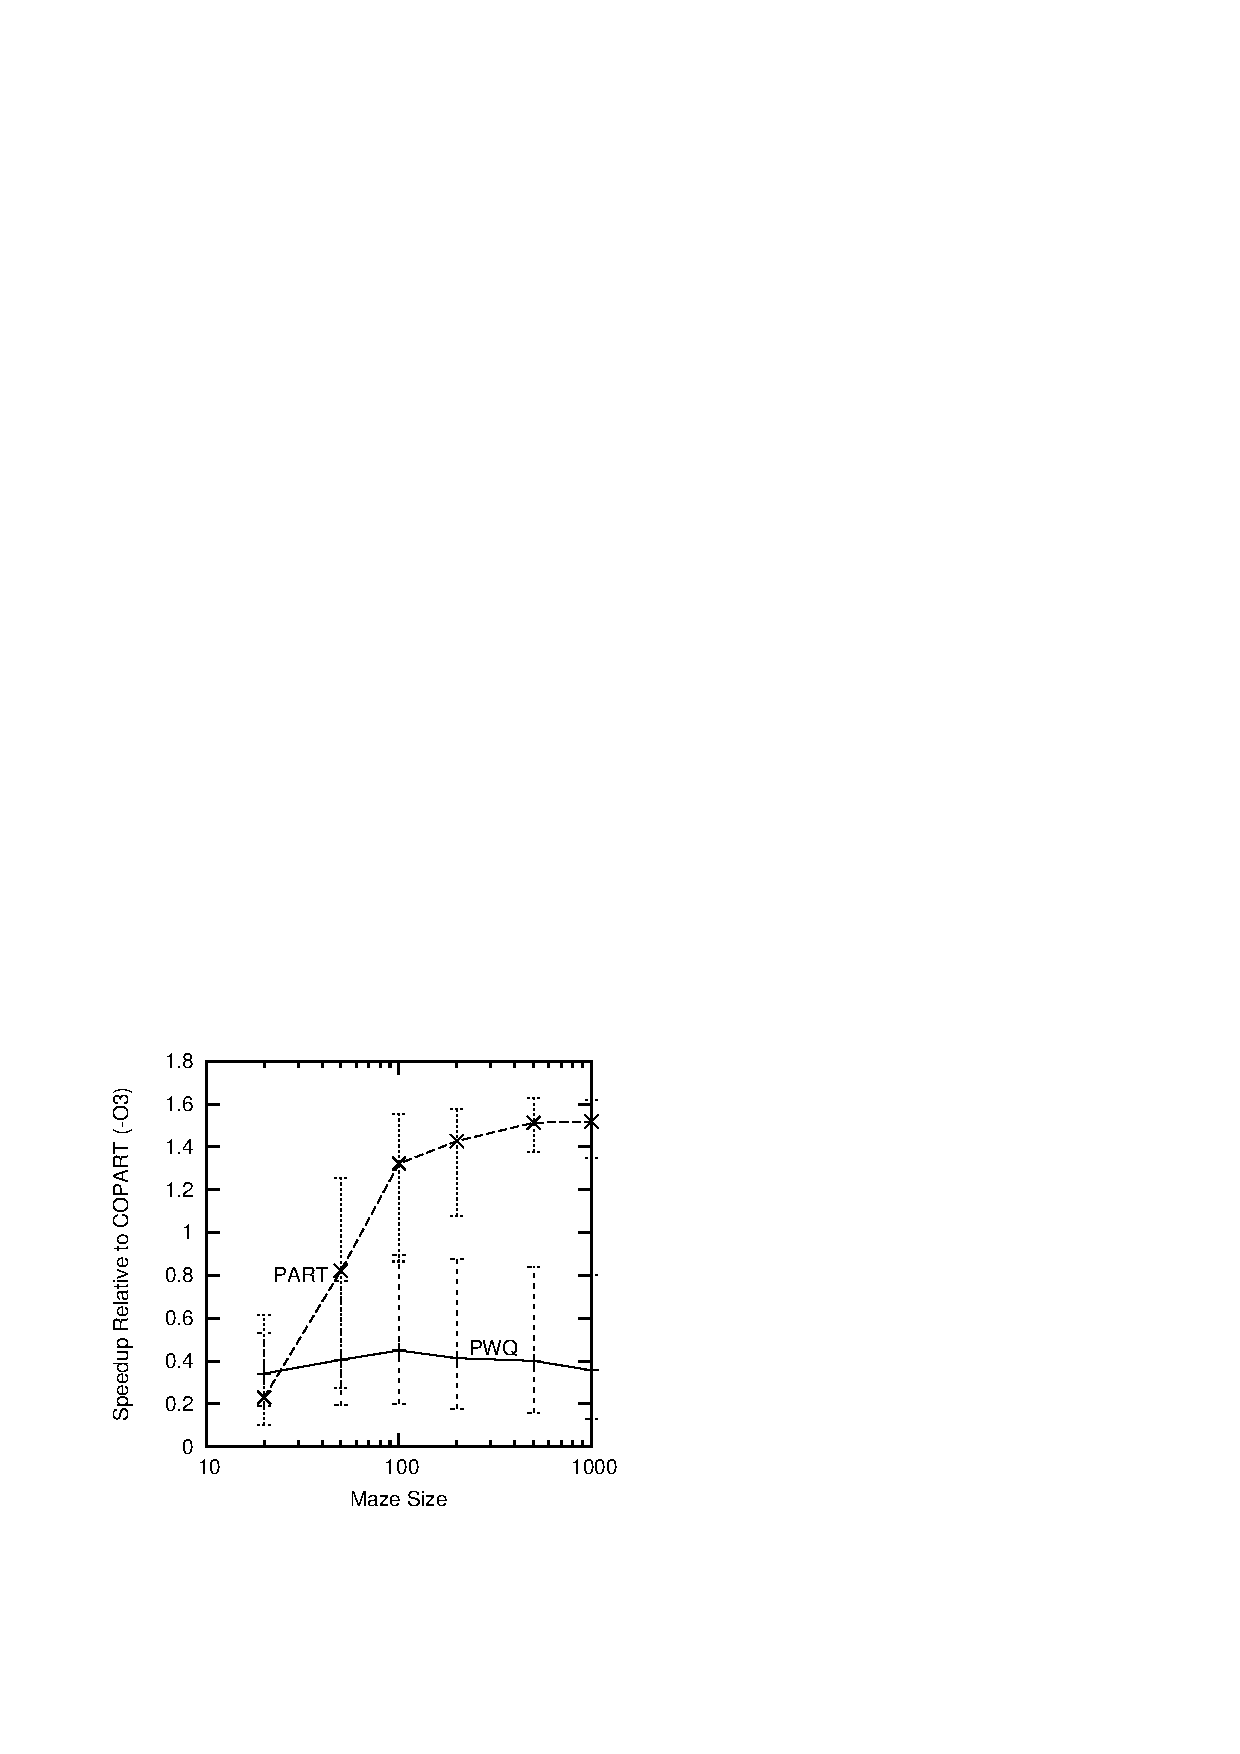
\includegraphics{SMPdesign/500-ms_2seqO3VfgO3_partO3-median}}
\caption{Varying Maze Size vs. COPART}
\label{fig:SMPdesign:Varying Maze Size vs. COPART}
\end{figure}

Figures~\ref{fig:SMPdesign:Varying Maze Size vs. SEQ}
and~\ref{fig:SMPdesign:Varying Maze Size vs. COPART}
show the effects of varying maze size, comparing both PWQ and PART
running on two threads
against either SEQ or COPART, respectively, with 90\=/percent\-/confidence
error bars.
PART shows superlinear scalability against SEQ and modest scalability
against COPART for 100-by-100 and larger mazes.
PART exceeds theoretical energy-efficiency breakeven against COPART at roughly
the 200-by-200 maze size, given that power consumption rises as roughly
the square of the frequency for high frequencies~\cite{TrevorMudge2000Power},
so that 1.4x scaling on two threads consumes the same energy
as a single thread at equal solution speeds.
In contrast, PWQ shows poor scalability against both SEQ and COPART
unless unoptimized: Figures~\ref{fig:SMPdesign:Varying Maze Size vs. SEQ} 
and~\ref{fig:SMPdesign:Varying Maze Size vs. COPART}
were generated using -O3.

\begin{figure}[tb]
\centering
\resizebox{2.2in}{!}{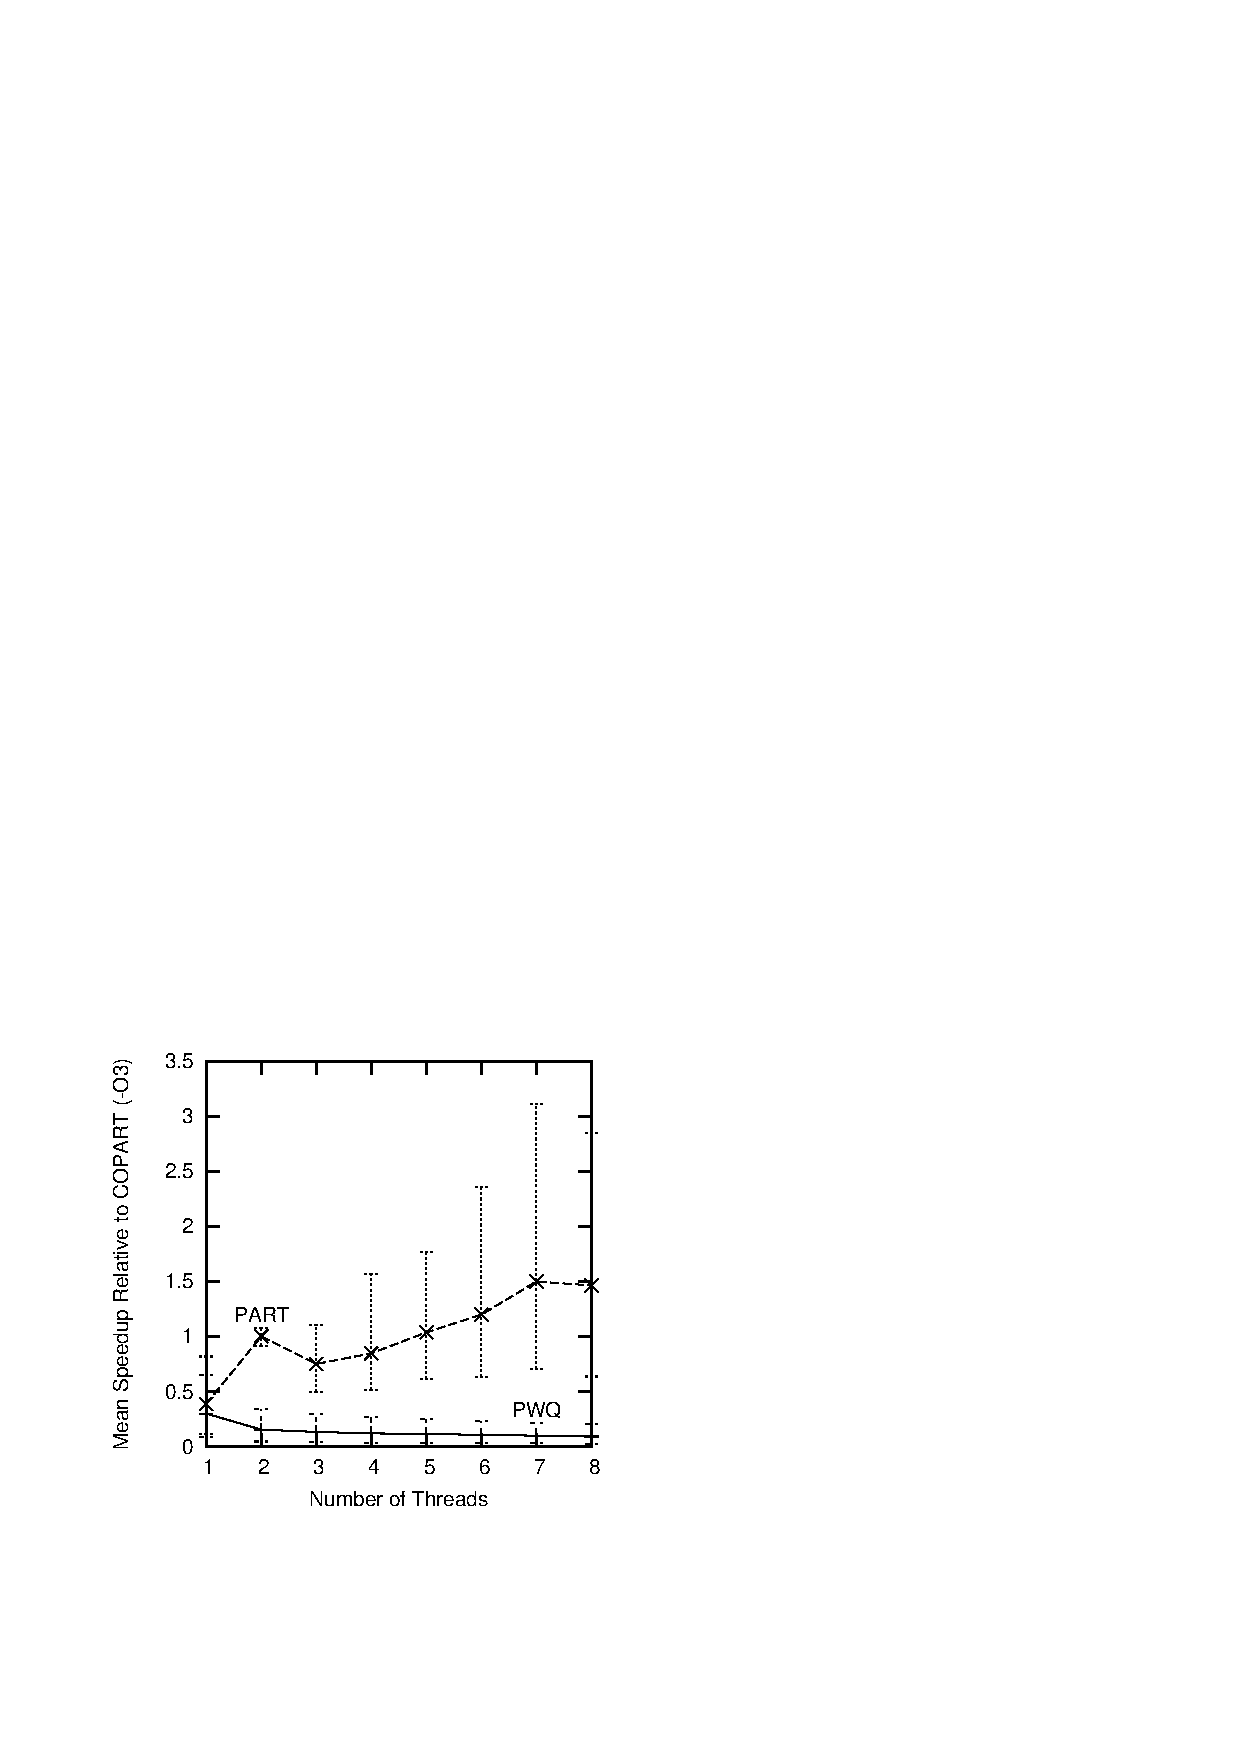
\includegraphics{SMPdesign/1000-ms_2seqO3VfgO3_partO3-mean}}
\caption{Mean Speedup vs. Number of Threads, 1000x1000 Maze}
\label{fig:SMPdesign:Mean Speedup vs. Number of Threads, 1000x1000 Maze}
\end{figure}

Figure~\ref{fig:SMPdesign:Mean Speedup vs. Number of Threads, 1000x1000 Maze}
shows the performance of PWQ and PART relative to COPART\@.
For PART runs with more than two threads, the additional threads were
started evenly spaced along the diagonal connecting the starting and
ending cells.
Simplified link-state routing~\cite{BERT-87} was used to
detect early termination on PART runs with more than two threads
(the solution is flagged when
a thread is connected to both beginning and end).
PWQ performs quite poorly, but
PART hits breakeven at two threads and again at five threads, achieving
modest speedups beyond five threads.
Theoretical energy efficiency breakeven is within the 90\=/percent\-/confidence
interval for seven and eight threads.
The reasons for the peak at two threads are (1) the lower complexity
of termination detection in the two-thread case and (2) the fact that
there is a lower probability of the third and subsequent threads making
useful forward progress: Only the first two threads are guaranteed to start on
the solution line.
This disappointing performance compared to results in
Figure~\ref{fig:SMPdesign:Varying Maze Size vs. COPART}
is due to the less-tightly integrated hardware available in the
larger and older Xeon system running at 2.66\,GHz.

\subsection{Future Directions and Conclusions}
\label{sec:SMPdesign:Future Directions and Conclusions}

Much future work remains.
First, this section applied only one technique used by human maze solvers.
Others include following walls to exclude portions of the maze
and choosing internal starting points based on the
locations of previously traversed paths.
Second, different choices of
starting and ending points might favor different algorithms.
Third, although placement of the PART algorithm's
first two threads is straightforward, there are any number of
placement schemes for the remaining threads.
Optimal placement might well depend on the starting and ending points.
Fourth, study of unsolvable mazes and cyclic mazes
is likely to produce interesting results.
Fifth, the lightweight C++11 atomic operations might improve performance.
Sixth, it would be interesting to compare the speedups for
three-dimensional mazes (or of even higher-order mazes).
Finally, for mazes, humiliating parallelism indicated a
more-efficient sequential implementation using coroutines.
Do humiliatingly parallel algorithms always lead to more-efficient
sequential implementations, or are there inherently humiliatingly parallel
algorithms for which coroutine context-switch overhead overwhelms the
speedups?

This section demonstrated and analyzed parallelization of maze-solution
algorithms.
A conventional work-queue-based algorithm did well only when compiler
optimizations were disabled, suggesting that some prior results obtained
using high-level/overhead languages will be invalidated
by advances in optimization.

This section gave a clear example where approaching parallelism
as a first-class optimization technique rather than as a derivative of a
sequential algorithm paves the way for an improved sequential algorithm.
High-level design-time application of parallelism is likely to be a
fruitful field of study.
This section took the problem of solving mazes from mildly scalable
to humiliatingly parallel and back again.
It is hoped that this experience will motivate work on parallelism
as a first-class design-time whole-application optimization technique,
rather than as a grossly suboptimal after-the-fact micro-optimization
to be retrofitted into existing programs.

\section{Partitioning, Parallelism, and Optimization}
\label{sec:SMPdesign:Partitioning, Parallelism, and Optimization}
%
\epigraph{Knowledge is of no value unless you put it into practice.}
	 {\emph{Anton Chekhov}}

Most important, although this chapter has demonstrated that applying
parallelism at the design level gives excellent results, this final
section shows that this is not enough.
For search problems such as maze solution, this section has shown that
search strategy is even more important than parallel design.
Yes, for this particular type of maze, intelligently applying parallelism
identified a superior search strategy, but this sort of luck is no
substitute for a clear focus on search strategy itself.

As noted back in Section~\ref{sec:intro:Parallel Programming Goals},
parallelism is but one potential optimization of many.
A successful design needs to focus on the most important optimization.
Much though I might wish to claim otherwise, that optimization might
or might not be parallelism.

However, for the many cases where parallelism is the right optimization,
the next section covers that synchronization workhorse, locking.
